\documentclass[conference]{IEEEtran}
\IEEEoverridecommandlockouts

% Package
\usepackage{cite}
\usepackage{amsmath,amssymb,amsfonts}
\usepackage{algorithm}
\usepackage[noend]{algpseudocode}
\usepackage{xcolor}
\usepackage{graphicx}
\usepackage{textcomp}
\usepackage{xcolor}

% Settings
%   1
\def\BibTeX{{\rm B\kern-.05em{\sc i\kern-.025em b}\kern-.08em
    T\kern-.1667em\lower.7ex\hbox{E}\kern-.125emX}}
%   2
\makeatletter
%	3
\newcommand{\linebreakand}{
  \end{@IEEEauthorhalign}
  \hfill\mbox{}\par
  \mbox{}\hfill\begin{@IEEEauthorhalign}
}
%   4
\makeatother
%   5
\pagecolor{white}

% ----- DOCUMENT STARTS HERE -----
\begin{document}

\title{Petification: Node-RED based Pet Care IoT Solution \\ using MQTT Broker}

\author{
    \IEEEauthorblockN{Haeram Kim}
    \IEEEauthorblockA{
        \textit{Computer Science and Engineering} \\
        \textit{Chungnam National University}\\
        Daejeon, Korea \\
        haeram.kim1@gmail.com
    }
    \and
    \IEEEauthorblockN{Hyejong Kang}
    \IEEEauthorblockA{
        \textit{Computer Science and Engineering} \\
        \textit{Chungnam National University}\\
        Daejeon, Korea \\
        kanghyejong1001@gmail.com
    }
    \and
    \IEEEauthorblockN{Sunghan Kim}
        \IEEEauthorblockA{
        \textit{Computer Science and Engineering} \\
        \textit{Chungnam National University}\\
        Daejeon, Korea \\
        seonghan.kim.cnu@gmail.com
    }
    \linebreakand
    \IEEEauthorblockN{Dukho Choi}
    \IEEEauthorblockA{
        \textit{International trade / software convergence} \\
        \textit{Chungnam National University}\\
        Daejeon, Korea \\
        dukho.fin@gmail.com
    }
    \and
    \IEEEauthorblockN{Jihyun You}
    \IEEEauthorblockA{
        \textit{Cybersecurity} \\
        \textit{Purdue University}\\
        West Lafayette, IN, USA \\
        you62@purdue.edu
    }
}

\maketitle 

% ----- ABSTRACT -----
\begin{abstract}
While there are an increasing number of households owning pets, it is challenging for owners who leave home often to take good care of their pets. The previous studies which are conducted to solve this problem use the free plan of paid IoT platform. As features which free plan of paid IoT platform supports are very limited, the proposed IoT solution named ‘Petification’ uses open-source IoT platform Node-RED with MQTT messaging protocol. In Petification, the water supplier and feed machine are attached to the platform to provide water and food to the pet and scale the weight of the water and food. The web-based dashboard is supported to show the remaining amount of water and food, show the water and food consumption, show the device connectivity, and serve the food by button or by schedule. The user of the Petification gets a notification when the water or food is running out of empty. The load cell, HX711 amplifier, and Raspberry Pi Zero W are mounted to the water supplier and feed machine to scale the water and food. In the feed machine, an MG90S servo motor is mounted to Raspberry Pi to serve the food to the pet. With Petification, users can take care of their pets remotely as well as check the device’s status. However, while serving the food to the pet, served amount mismatches with the desired amount. Thus, the future plan can be enhancing the food gate to serve the exact amount of food and the solution by adding more devices. \\
\end{abstract}

% ----- KEYWORD -----
\begin{IEEEkeywords}
IoT platform, Node-RED, MQTT, Smart pet care service 
\end{IEEEkeywords}

% —— INTRODUCTION ——
\section{Introduction}
% `Project background`
As the number of households living alone increases and the culture of raising pets spreads compared to the past, the number of households raising pets is increasing. This trend is shown in the growth of the pet industry; The profit of the pet industry is more than doubled every year over 10 years, from \$48.4 billion in 2010 to \$109.6 billion in 2020 \cite{b1}. Along with this trend, demand for tracking pet wellness is increased accordingly. One of the demanded services is tracking a pet’s status when the pet is left alone. Because for those who left home often, it is challenging to take good care of their pets.

% `Problem statement`
As a way to solve this problem, Internet of Things (IoT) technology has emerged. A lot of pet care IoT solutions are introduced in the market, and many studies and implementations are suggested.
However, the IoT platforms which are used to implement pet care IoT solution has limitations. For example, a most commonly used IoT platform is "Blynk" \cite{b2, b3, b4, b5}, but the latest version of it is not an open-source and open-source version is no longer maintained. Also, "Adafruit IO" \cite{b6} and "Freeboard IO" \cite{b7} are another commonly used IoT platform, but they are not open-source.
Moreover, while tracking water and food consumption and automatic feeding are commonly supported by previous implementations, there are few solutions that support device status information and error notification.

% `Project novelty`
The proposed IoT solution named "Petification" uses open-source projects for IoT platform. Node-RED which is a flow-based open-source visual programming tool \cite{b8} is used to implement the APIs of the IoT platform. By using Node-RED, Petification can get the benefit of providing user-friendly UI, fast development, and a lot of resources shared by users. Also, Eclipse Mosquitto which is one of the open-source implementation of the MQTT messaging protocol is used to manage overall message flow. Using MQTT protocol as a message broker allows the IoT platform to connect user with devices in lightweight way \cite{b9}.

% `Functionality`
Petification provides informations about device connectivity and amount of remaining  food/water for each device as well as food/water consumption. Additionally, Petification provides an error notification service when the water or food is running out of empty among with automatic feeding service.
The water supplier and feed machine are attached to the platform to feed and water to the pet and to scale the weight of the food/water. While both water supplier and feed machine uses the load cell to scale the weight, a servo motor is attached only to the feed machine so that the user can control the served amount of food. All the load cells and servo motors are mounted to Raspberry Pi for each device.
The web-based dashboard is supported to show the remaining amount of water and food, show the water and food consumption, show the device connectivity, and serve the food by button or by schedule. The user of the Petification gets a notification when the water or food is running out of empty.

% —— Literature Review ——
\section{Related Literature}
% Index paragraph
This chapter will be explained with hardware and software perspectives respectively. In the hardware part, used devices are compared with them of Petification, and used IoT platform and provided feature will be compared with present research in the software part.

\subsection{Hardware}
% Reference 1
P. N. Vrishanka \textit{et al.} \cite{b10} proposed an automated pet feeder which serves food to the pet according to the remaining amount of food in the food bowl. An ultrasonic distance sensor and SG90 servo motor were mounted to Arduino Uno R3 in this research. An ultrasonic distance sensor is used to determine the remaining food amount by measuring the distance from the entrance of the feed container to the inside of the bowl.

% Comparison
However, the feed machine of Petification used load cell sensors to determine the remaining food amount, as it is difficult to use ultrasonic waves to measure the amount of feed accurately.

% Reference 2, 3
Rogerio Nogueira \textit{et al.} \cite{b11} proposed a system that provides food and water to the pet, takes pictures of the pet, and provides an intelligent interface to the user with the messenger. In this research, a rotary valve and DC motor were used to provide food to the pet. Vania \textit{et al.} \cite{b12} proposed an IoT solution that provides RFID to identify the pet, serves food by schedule, and provides an application to the user. This research also uses a propeller blade and DC motor for remote feeding.

% Comparison
However, the problem with using a rotary valve or propeller blade is that the feed can’t be provided with the exact weight. This is because the amount of feed to be provided to the pet is determined based on the serving unit contained in one space. Thus, when the feed machine tries to provide certain weight of feed with the rotary valve or propeller blade, there is always the possibility of providing more than the intended weight, even if the error for load cell is not concerned. The Petification feed machine does not use a rotary valve but uses a gate that can block the feeder container outlet because it has the advantage of being able to adjust the amount of feed to be supplied in more detail than the rotary valve method.

In addition, both \cite{b11} and \cite{b12} uses a DC motor to provide feed through continuous rotation of the rotary valve. However, the feed machine of Petification uses a servo motor because they need more precise control than free continuous rotation \cite{b13}.

\subsection{Software}
% Reference 4
Y. Chen \textit{et al.} \cite{b5} proposed a pet care IoT system that provides food and water consumption, the number of defecation, and defecation duration. It was developed through Arduino IDE and provides features above with numbers and visual statistics in real-time using “Blynk” as an IoT platform.

% Reference 5
T. Sangvanloy \textit{et al.} \cite{b4} proposed a pet care IoT solution that visualizes the daily food consumption in real-time and automatically feeds the pet according to the scheduled time. It was also implemented using “Blynk” as an IoT platform.

% Platform Comparison
From the used platform perspective, the above two studies commonly used ‘Blynk’ as an IoT platform. However, Petification uses Node-RED instead of ‘Blynk’ to take advantage of visual programming, openly pre-developed flows and nodes, and various notification means.

% Functionality Comparison
Also, non of the two studies above provide information on device status. Although tracking water and feed consumption is an important feature in pet care IoT solutions, keeping track of IoT devices’ status is also an important feature. Petification provides the status of feed machines and water supply machines, such as device connectivity, error existence, and the amount of feed or water remaining in the device. Moreover, Petification provides an error notification feature that notifies users when the error occurred, such as when water or feed is empty.

% —— METHODOLOGY ——
\section{Methodology}
% Section Index
In this chapter, the overview and used technologies are explained. The high-level outline of Petification is explained in the overview part, and used technology including sensor, actuator, program, and protocol is explained in the technology part.

\subsection{Overview}
As MQTT is the main messaging protocol for Petification and MQTT uses TCP/ IP protocol stack, each device is connected to the Access Point (AP) through Wi-Fi. Thus, all the messages published from devices are sent to the AP with Wi-Fi, and then they are sent to the Petification platform through the internet. Petification platform processes the messages and sends the processed data to the users in form of a web dashboard page, E-Mail, and WhatsApp messages. On the contrary, users can send requests with the web dashboard to the platform. While some requests require only the platform, the requests to activate the actuator are forwarded to the device with the help of the platform. In summary, users and devices communicate bi-directionally through the platform. The overview for Petification is shown in figure 2.

% `Overview.png`
\begin{figure}[htbp]
\centerline{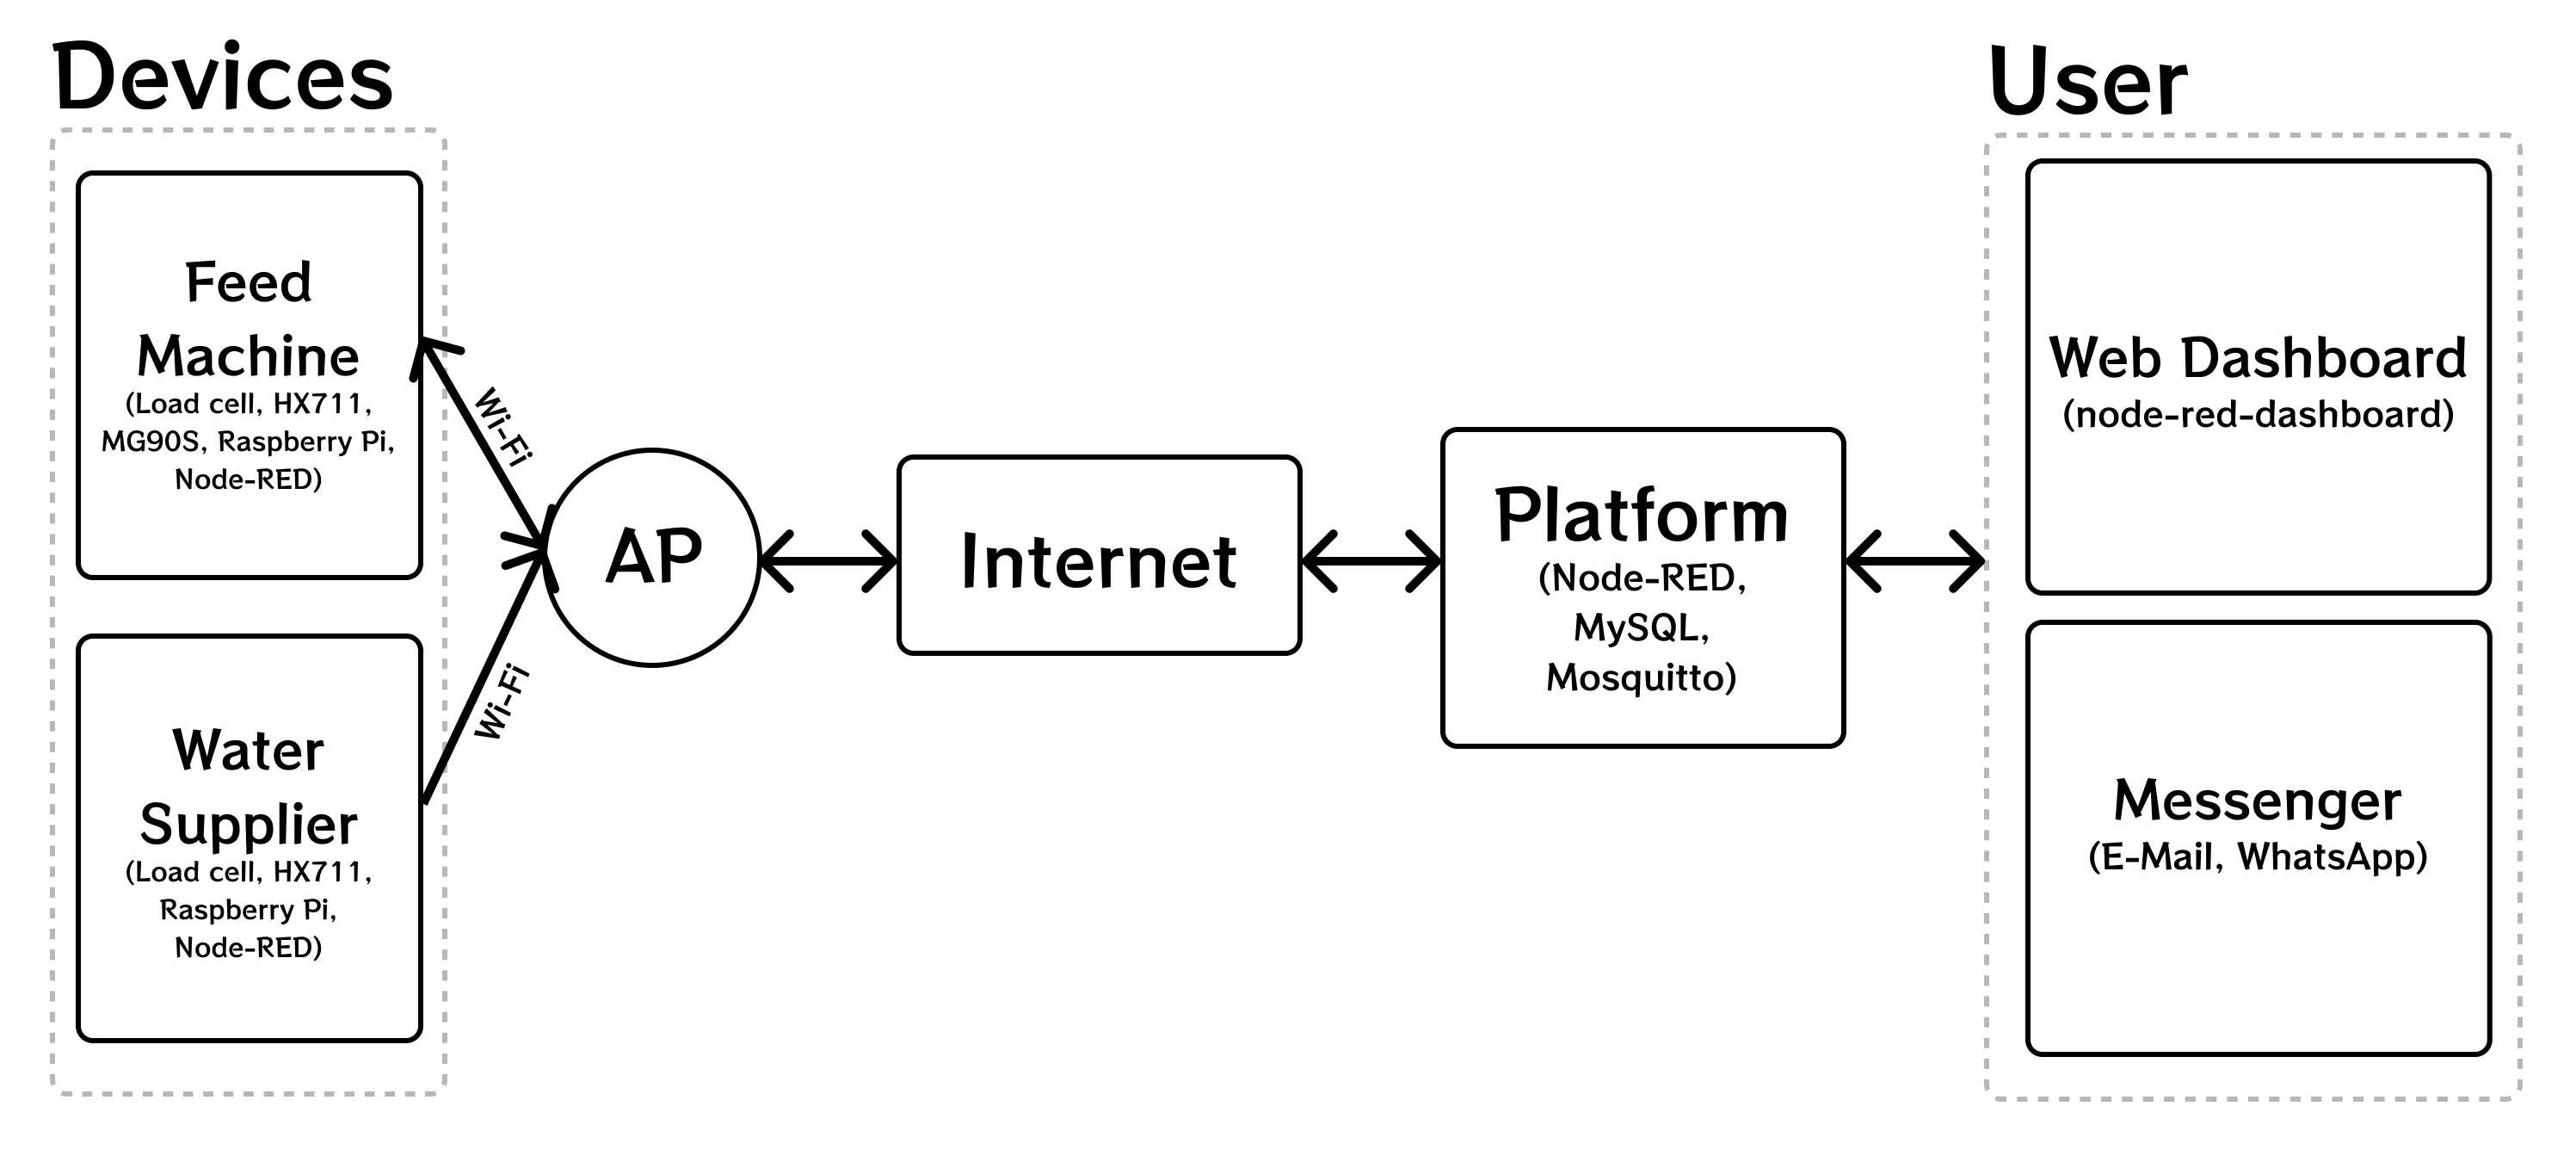
\includegraphics[width=0.5\textwidth]{./images/Overview.png}}
\caption{Petification overview}
\label{fig}
\end{figure}

\subsection{Used Technology}
\subsubsection{Hardware}
% ::Load cell::
The load cell sensor serves to convert the weight or force acting into an electrical analog signal \cite{b14}. In the present research, three load cells that can weigh up to 5kg with 1g accuracy are used.
% ::HX711 Amplifier::
All the load cells are mounted to the microcontroller through a load cell amplifier. In Petification, three HX711 modules are used as load cell amplifiers. HX711 converts an analog signal into a digital signal, amplifies a measured value of a low load cell, and then transmits the value to another microcontroller \cite{b15}. 
% ::MG90S Servo Motor::
The servo motor is a rotary or linear actuator that rotates and pushes a machine \cite{b16} and one MG90S servo motor is used.
% ::Raspberry Pi Microcontroller::
The role of the microcontroller is orchestrating all the sensors and actuators and communicating with the IoT platform. For the microcontroller, two Raspberry Pi Zero W are used.

\subsubsection{Node-RED}
% ::1. Flow-based visual development tool - fast development::
Node-RED is a flow-based visual development tool that is easy for developers and non-developers to develop programs \cite{b17}.
% ::3. IBM-supported open source::
It is originally developed by International Business Machines Corporation (IBM), and IBM made it to an open-source project in 2013 \cite{b8}. Not only Node-RED itself but also various nodes are being distributed through Node Package Manager (NPM). Thus, users can share their nodes or flows, and a lot of contributed nodes are available in NPM.
% ::2. Interoperability::
One of the Node-RED’s operational strengths is that it can run on various environments such as local, Raspberry Pi, Docker, Cloud Instance, \textit{et al.} Thus, Node-RED v2.2.1 is installed in not only the platform server but also Raspberry Pi of water supplier and feed machine.

\subsubsection{MQTT}
MQTT stands for Message Queuing Telemetry Transport. It is an OASIS standard protocol and provides light-weight, publish/subscribe messaging transport for IoT \cite{b9}.
% ::Light-weight::
One characteristic of MQTT is light-weight. The MQTT protocol has a small message size and message overhead and consumes less power and resources than Advanced Message Queuing Protocol (AMQP) and Hypertext Transfer Protocol (HTTP) \cite{b18}. With its light-weight characteristic, it is suitable for communication in IoT fields where network bandwidth is at a premium \cite{b19}.
% ::Reliability::
MQTT uses TCP as transport layer protocol and TLS/SSL can be used for security. It makes MQTT more reliable than Constrained Application Protocol (CoAP) which uses UDP as the transport protocol \cite{b18}.
% ::Pub/sub::
All MQTT messages have their own topics, and MQTT clients can send data for a certain topic by publishing messages to MQTT broker or receive data by subscribing to topics for those messages.
% ::Mosquitto::
In this research, Eclipse Mosquitto v1.4.15 is used as an MQTT Message Broker. Eclipse Mosquitto is an open-source message broker implementing MQTT protocol versions 5.0, 3.1.1, and 3.1\cite{b20}. 

\subsubsection{MySQL}
MySQL is a fast, flexible, and easy-to-use database with RDBMS (relational database management system). The combination of MySQL’s secure processing and reliable software provides effective transactions for large projects, so it is flexible with open sources. MySQL is also excellent in terms of data security because it is evaluated as having the safest and most reliable database management system \cite{b21}. In addition, MySQL is considered a suitable database to manage effective data flows because it has good compatibility with Node-RED \cite{b21}. The used version of MySQL is v5.7.37.

% —— HARDWARE DESIGN ——
\section{Hardware Design}
\begin{figure}[htbp]
\centerline{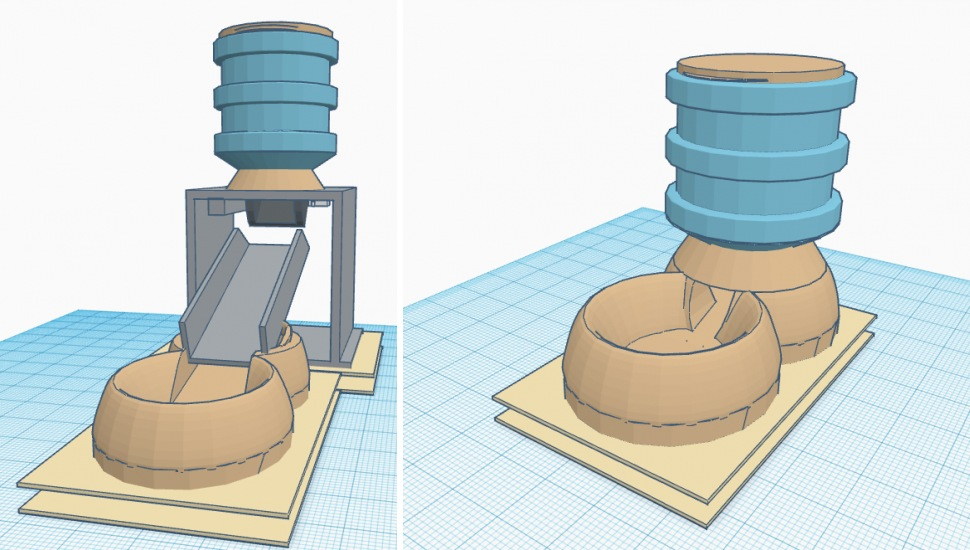
\includegraphics[width=0.5\textwidth]{./images/Feed Machine & Water Supplier.jpg}}
\caption{CAD design for the feed machine and water supplier}
\label{fig}
\end{figure}

\subsection{Feed Machine}
Feed Machine is one of the devices attached to the proposed platform. The Feed Machine has 2 main functionalities: serving food to the pet and publishing the weight of the food bowl and container to the platform. To serve food to the pet, the servo motor is mounted to open and close the food gate. As in figure 4, the servo motor gives food in an open/close type. Food serving is done with the help of gravity; After the food gate is opened, food rolls down the slope, and thus food is served. By closing the food gate Feed Machine stops the serving of the food. To measure the weight of the food bowl and container, two load cell is mounted under each of them. Like in figure 5, each load cell is connected with an HX711 Amplifier to convert the analog signal to a digital signal. Also, as in figure 3, Load cell sensors are installed between wooden boards to measure the weight. Additionally, in figure 3, a food container carries food through a slide into a food bowl. All the sensors and a servo motor are attached to Raspberry Pi Zero W.

\begin{figure}[htbp]
\centerline{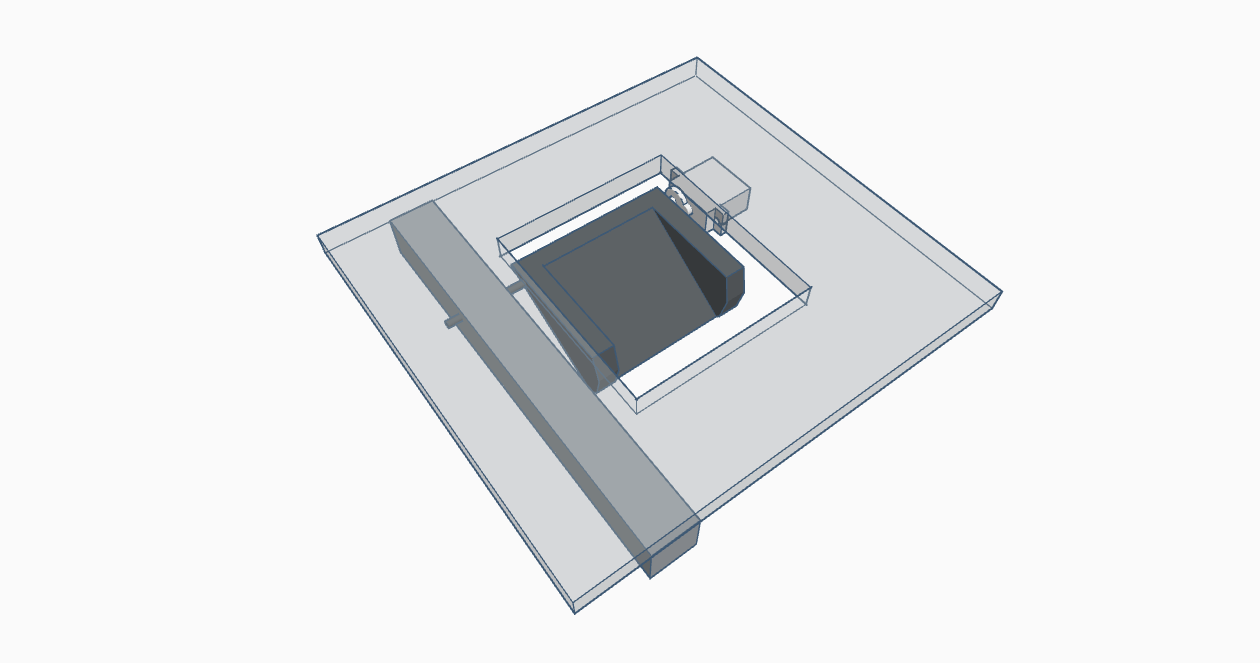
\includegraphics[width=0.5\textwidth]{./images/servo_gate.png}}
\caption{Food gate of the feed machine}
\label{fig}
\end{figure}

\begin{figure}[htbp]
\centerline{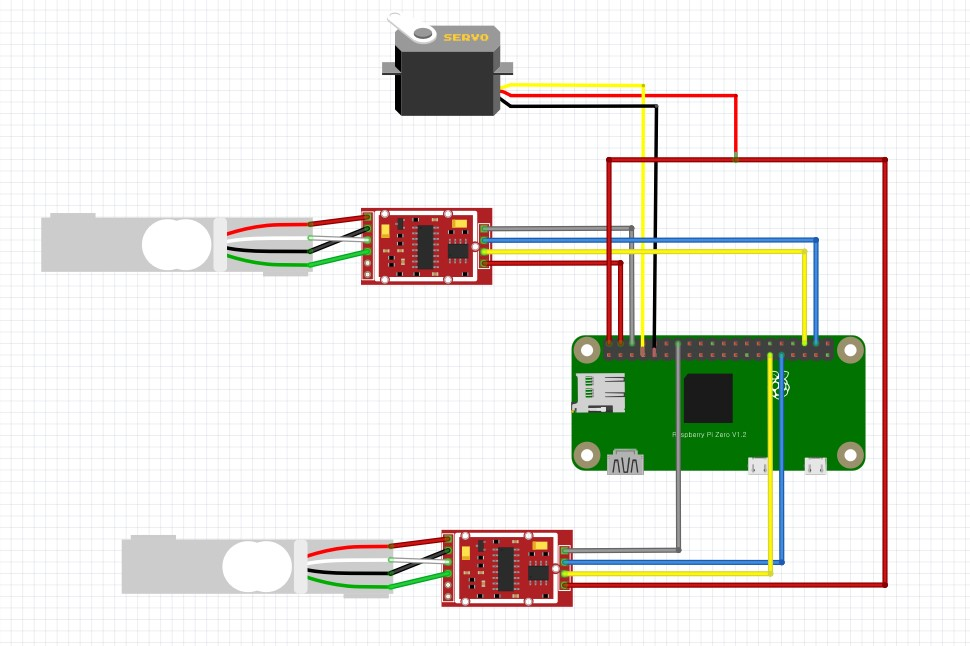
\includegraphics[width=0.5\textwidth]{./images/feed machine circuit.jpg}}
\caption{Circuit diagram of the feed machine}
\label{fig}
\end{figure}

\subsection{Water Supplier}
The water supplier is also a device attached to the proposed platform. The main functionalities for the water supplier are supplying the water to the pet and publishing the weight of the remaining water. However, a servo motor is not used for the water supplier as controlling the serving amount of the supplied water isn’t necessary. Similar to a feed machine, to measure the weight of water in a water supplier a load cell is mounted under the water supplier. In addition, like in figure 6, the HX711 amplifier is used to convert analog signals into digital signals. As in figure 3, like a feed machine load cell sensors are installed between wooden boards to measure the weight. Both types of sensor and RaspberryPi are the same as the feed machine. 

\begin{figure}[htbp]
\centerline{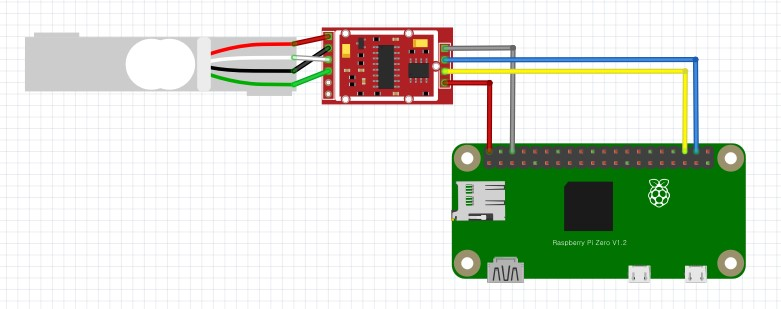
\includegraphics[width=0.5\textwidth]{./images/water supplier circuit.jpg}}
\caption{Circuit diagram of the water supplier}
\label{fig}
\end{figure}

% —— SOFTWARE DESIGN ——
\section{Software Design}
\subsection{User-to-device communication}
\begin{figure}[htbp]
\centerline{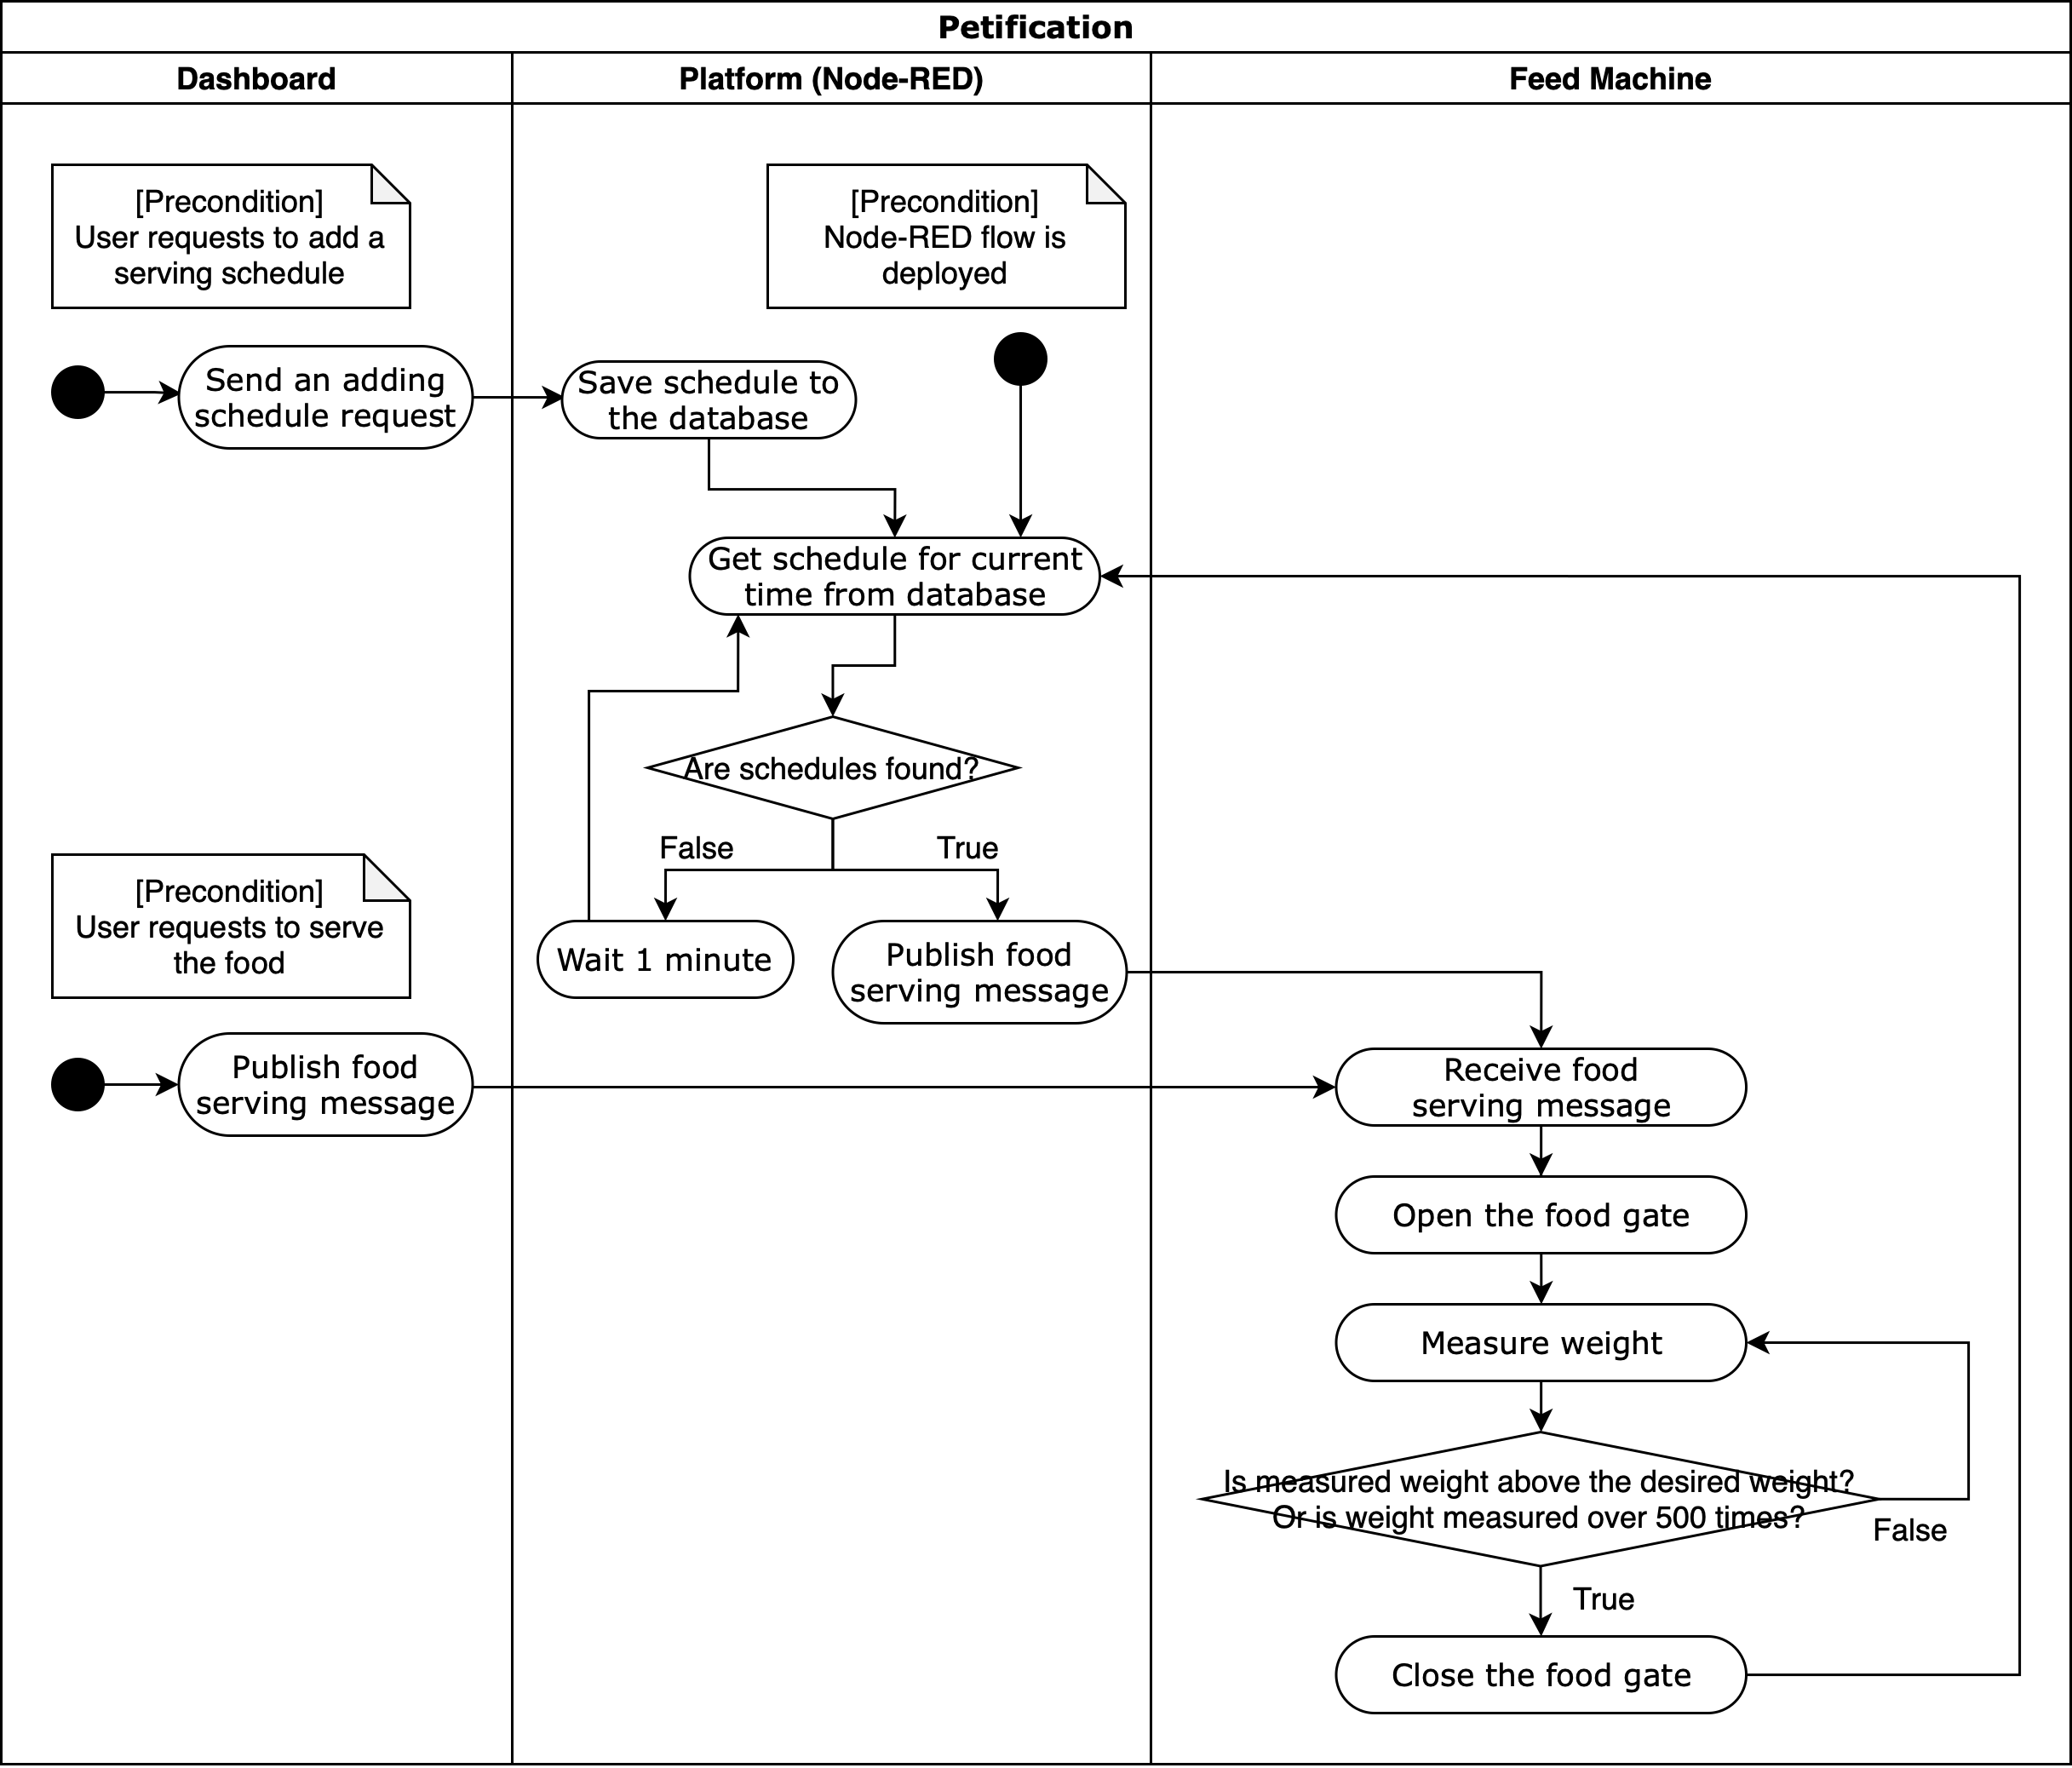
\includegraphics[width=0.5\textwidth]{./images/user2device.png}}
\caption{Activity diagram for user-to-device communication}
\label{fig}
\end{figure}
% ::Publish action message::
As shown in figure 7, serving a certain amount of food is done in user-to-device communication. When the Node-RED flow of the platform is deployed or when the user adds a schedule to the database, the platform selects the schedules which are supposed to be activated at the current time from the database. The food serving messages are published only when corresponding schedules are found in the database. When the schedules are not found, the platform waits 1 minute and does the same job again. The food serving message is also published when the user manually requests to serve the food.

% ::Serve the food::
As the feed machine is a subscriber for the food serving message, the food serving message is sent to the feed machine. When the feed machine receives the food serving message, it opens the food gate to serve the food. And the feed machine repeatedly measures the weight of the food bowl. The food gate of the feed machine is closed when the measured weight is above the desired weight or when the device measures the weight over 500 times. After the food gate of the feed machine is closed, the platform inquires another schedule for the current time from the database repeatedly.

\subsection{Device-to-user communication}
\begin{figure}[htbp]
\centerline{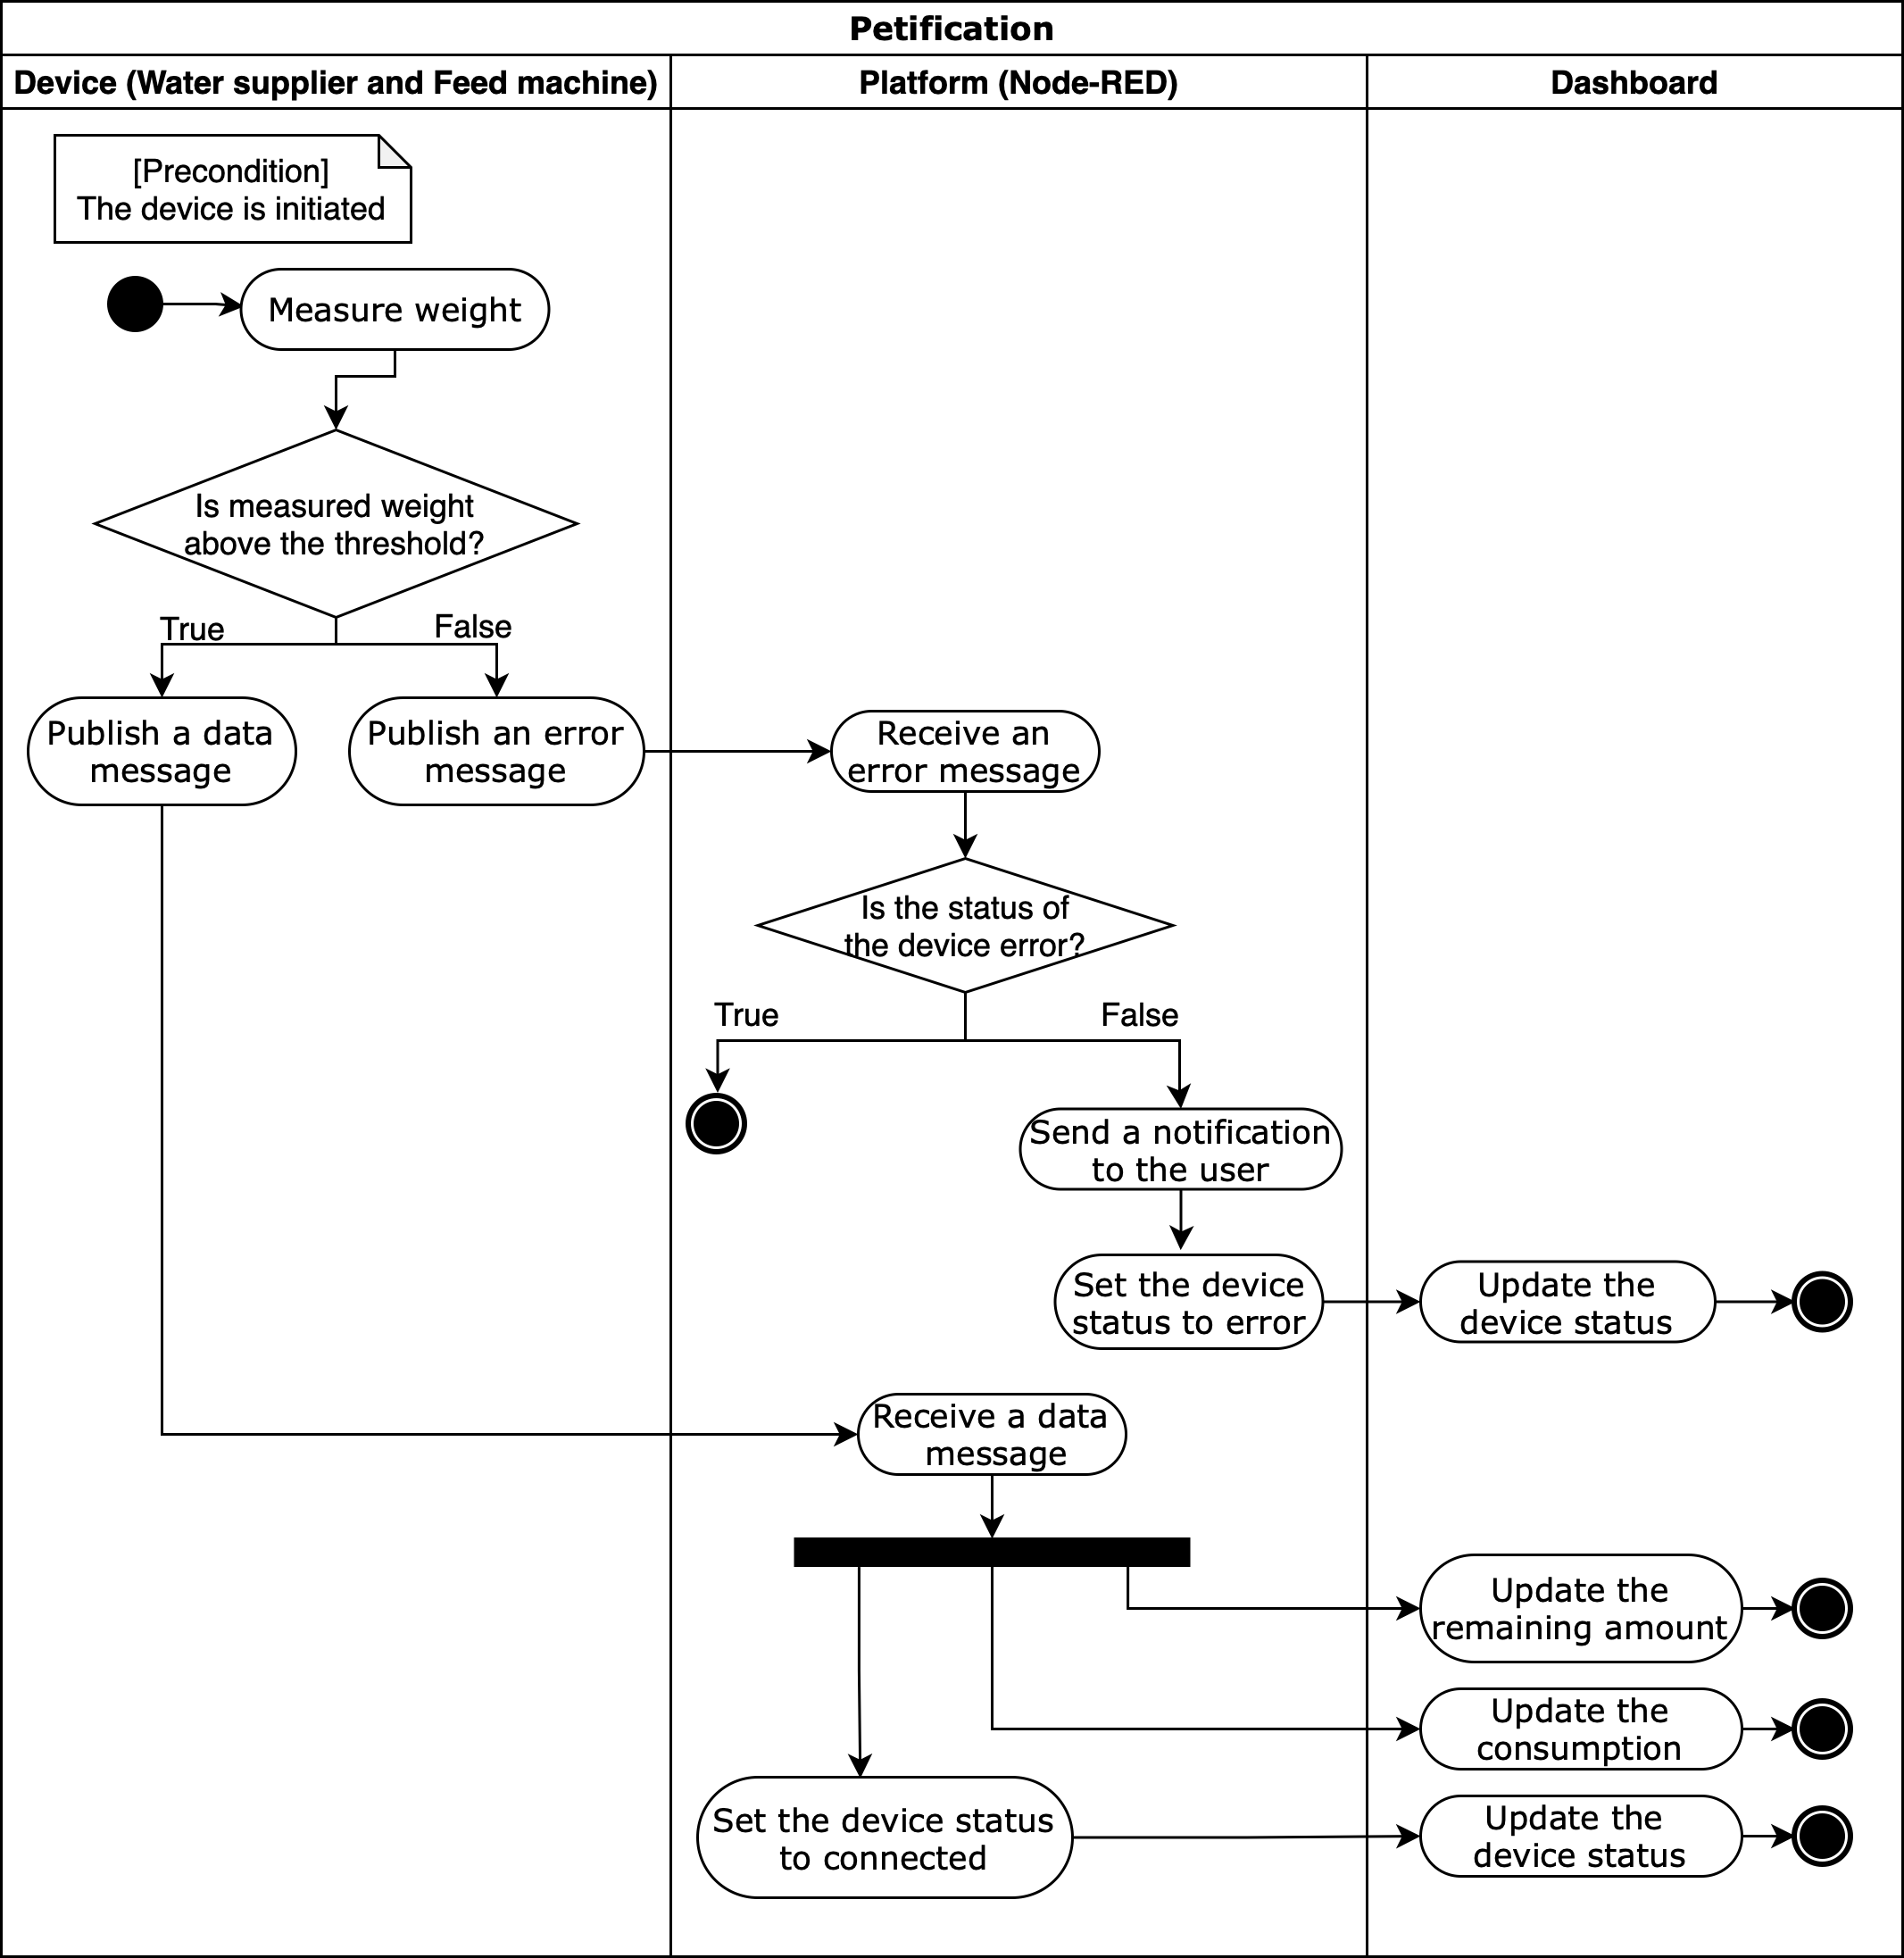
\includegraphics[width=0.5\textwidth]{./images/device2user.png}}
\caption{Activity diagram for device-to-user communication}
\label{fig}
\end{figure}

% ::Publish scale message::
The flow shown in figure 8 is done repeatedly to figure out the weight of the water or food which each device contains. In each flow, the water supplier and feed machine measure the weight. When the measured weight is above the threshold which is a criterion of knowing whether the water or food is empty, a data message that contains measured weight is published. However, if it is not, an error message is published. 

% ::Receive scale message::
When the platform which is a subscriber for data message receives the data message, it sets the status of the device to ‘connected’ which means the device is working correctly. And it updates the dashboard to provide the remaining amount and consumption of the water or food to the user in a visual way. The consumption is calculated by adding the decreased amount to the previous consumption. The pseudo-code for calculating the consumption is shown in algorithm 1.

\begin{algorithm}
\caption{Calculate consumption}\label{algo}
\begin{algorithmic}[1]
    \Procedure{CalcConsumption}{}
        \State $prevConsumption \gets \text{previous } \textit{consumption}$
        \State $currScale \gets \textit{scale} \text{ of received message}$
        \State $prevScale \gets \textit{scale} \text{ of  previous record}$
        \State $decrease \gets 0$
        \If{$precScale \neq \textit{null} \And prevScale > currScale$}
            \State $decrease \gets prevScale - currScale$
        \EndIf
        \Return $prevConsumption + decrease$
    \EndProcedure
\end{algorithmic}
\end{algorithm}

% ::Receive scale message::
As the platform subscribes to the error message, the error message is sent to the platform. When the error message is received, the platform selects the status of the device from the database. While the error message is ignored If the status of the device is ‘error’, the platform sends the notification to the user about the received error when the status is not ‘error’. After the notification is sent, the status of the device is changed to ‘error’ and the dashboard is updated accordingly.

% —— IMPLEMENTATION ——
\section{Implementation}

% ::—— Hardware Implementation ——::
\subsection{Hardware}
% ::Implantation result for both devices::
The result of the implementation for the water supplier is shown in figure 9, and that for the feed machine is shown in figure 10.

% ::Water supplier::
\begin{figure}[htbp]
\centerline{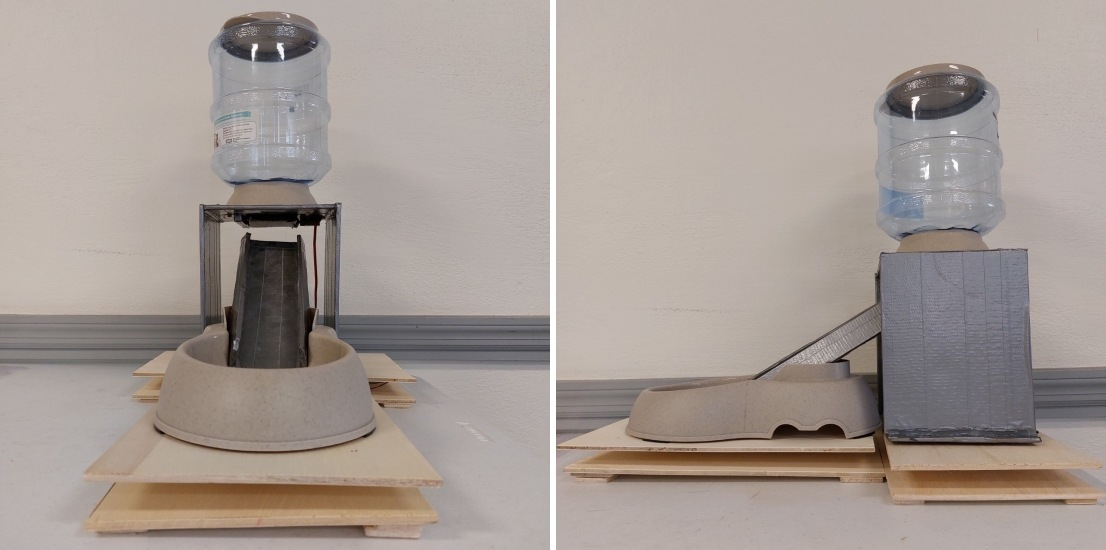
\includegraphics[width=0.5\textwidth]{./images/Water Supplier.jpg}}
\caption{Result of implementation for water supplier}
\label{fig}
\end{figure}

% ::Feed Machine::
\begin{figure}[htbp]
\centerline{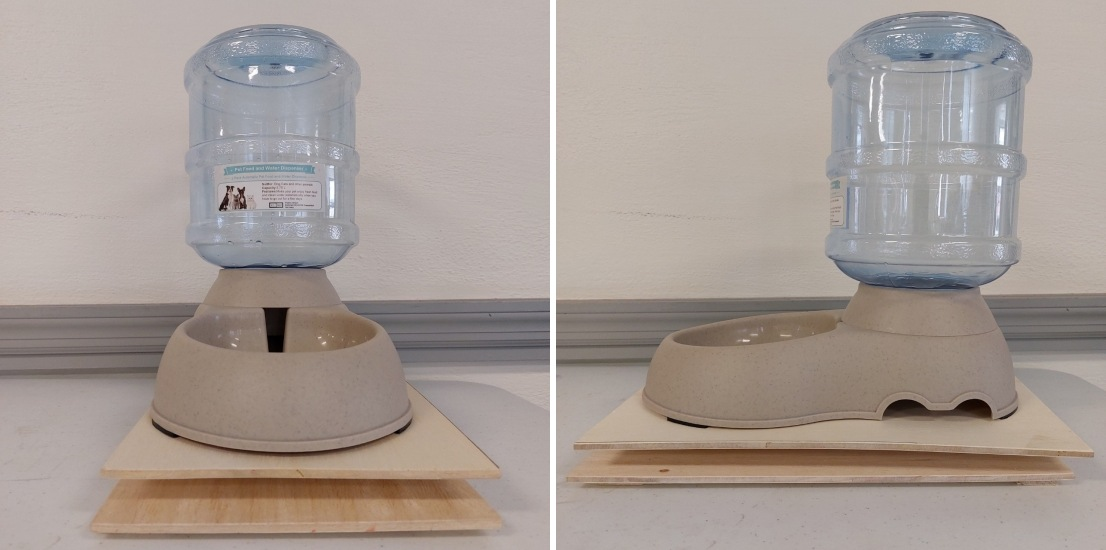
\includegraphics[width=0.5\textwidth]{./images/Feed Machine.jpg}}
\caption{Result of implementation for feed machine}
\label{fig}
\end{figure}

% ::Calibration and Weight measurement::
\subsubsection{Calibration and weight measurement}
% ::Calibration::
To convert the measurement of the load cell to the weight data, the calibration process has proceeded to get the reference unit. The process of calibration takes two steps. First, the force acting on the load cell by a standard object of known weight is repeatedly measured. In the calibration process of the petification, a 500mL bottle of water is used as a standard object for 500g weight. Second, get a reference unit by calculating the average measurement of the standard object and dividing it by actual weight, which is 500g in this case.

% ::Weight Measurement::
Measuring the weight of the water and food is done with python code. By using the ‘exec’ node of the Node-RED in Raspberry Pi to execute python code, the result of a measurement can be used in Node-RED. However, even if the calibration has proceeded, there is always the possibility of measurement error. Thus the ’smooth’ node of the ‘node-red-node-smooth’ library has been used to get a maximum value of two measurement results. By calibrating the measurement and calculating the maximum value, each Raspberry Pi in the water supplier and feed machine can get the correct weight.

% ::Publishing weight or error message::
\subsubsection{Publishing weight or error message}
Before publishing the weight of the water and food, the error detecting process has been progressed with using the ’switch’ node of the Node-RED. The ‘switch’ node checks if the weight is below the threshold value which is 10g for this implementation. When it’s true, each device publishes an error message instead of a scale message. Error message and scale message is distinguished by topic and payload of the message is either error message or weight value. The implemented Node-RED flow for publishing weight or error messages is shown in figure 11.

\begin{figure}[htbp]
\centerline{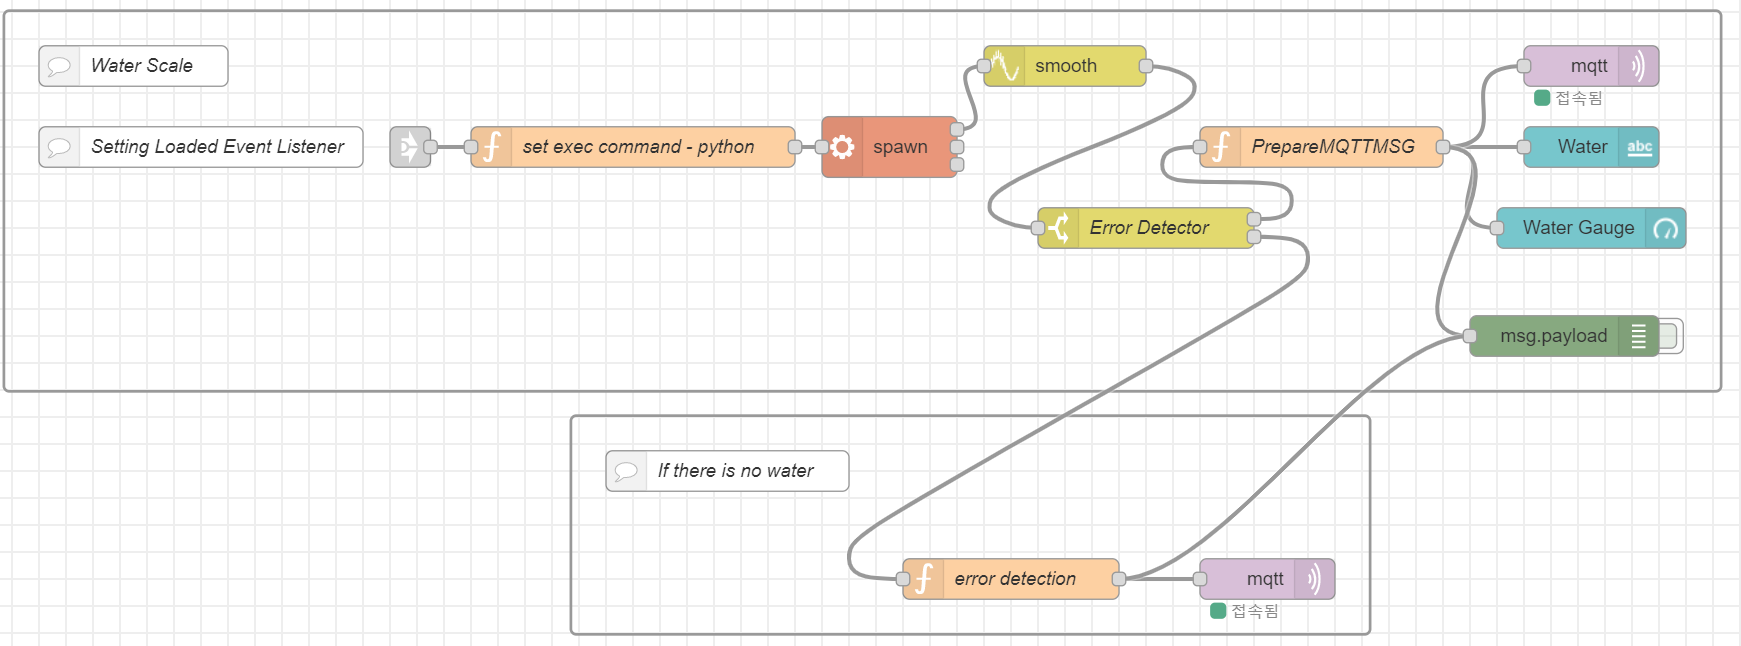
\includegraphics[width=0.5\textwidth]{./images/Water Supplier Error Detection.png}}
\caption{Node-RED screenshot for publishing weight or error message}
\label{fig}
\end{figure}

% ::Automatic feeding::
\subsubsection{Automatic feeding}
The action message is structured to contain ‘action’ in the message topic and desired serving amount in the message payload. When an action message has arrived, the bowl’s weight and message payload which is desired food weight are combined into one message. It is sent to a ‘loop’ node that is supported by the ‘node-red-contrib-loop-processing’ library and if the index is 0 and the bowl weight is less than the user’s input, the container’s servo motor opens the door to provide food. It continues to compare the two weights, the bowl weight is measured, and the payload of the message sent is continuously updated. During the loop, when the bowl weight becomes bigger than the user’s input, the loop ends and the servo motor closes the door and ends feeding. The implemented Node-RED flow for automatic feeding is shown in figure 12.

\begin{figure}[htbp]
\centerline{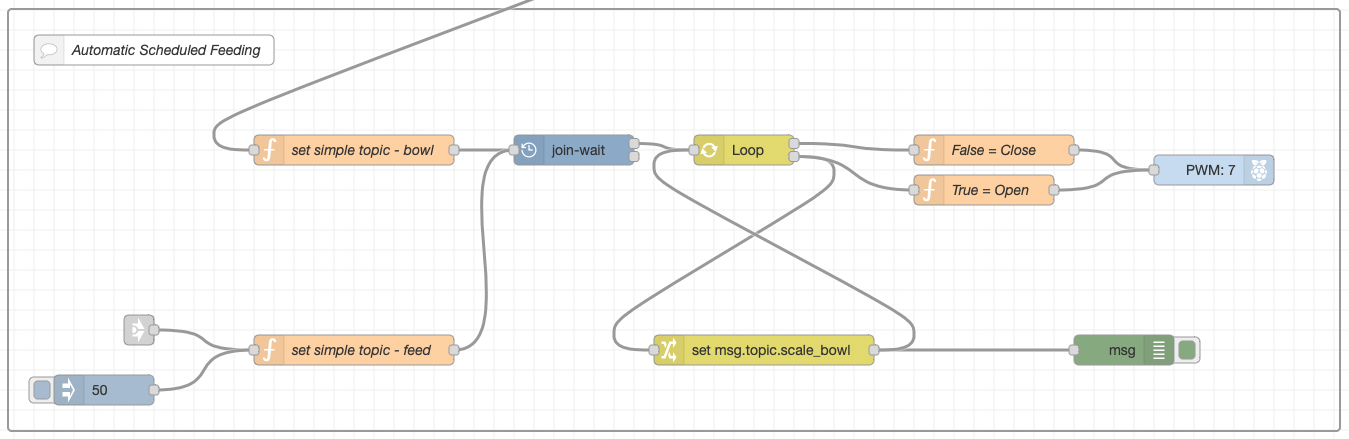
\includegraphics[width=0.5\textwidth]{./images/automaticFeeding.png}}
\caption{Node-RED screenshot for automatic feeding}
\label{fig}
\end{figure}

% ::—— Software Implementation ——::
\subsection{Platform}
The platform for Petification uses cloud instances for deployment. On the cloud instance, Mosquitto, MySQL, and Node-RED are installed and firewall, DNS, and certificate for TLS/SSL communication are configured for networking. In the Node-RED, 7 blocks are implemented as 7 flows. The screenshot for implemented Node-RED flow is shown in Figure 13.

\begin{figure}[htbp]
\centerline{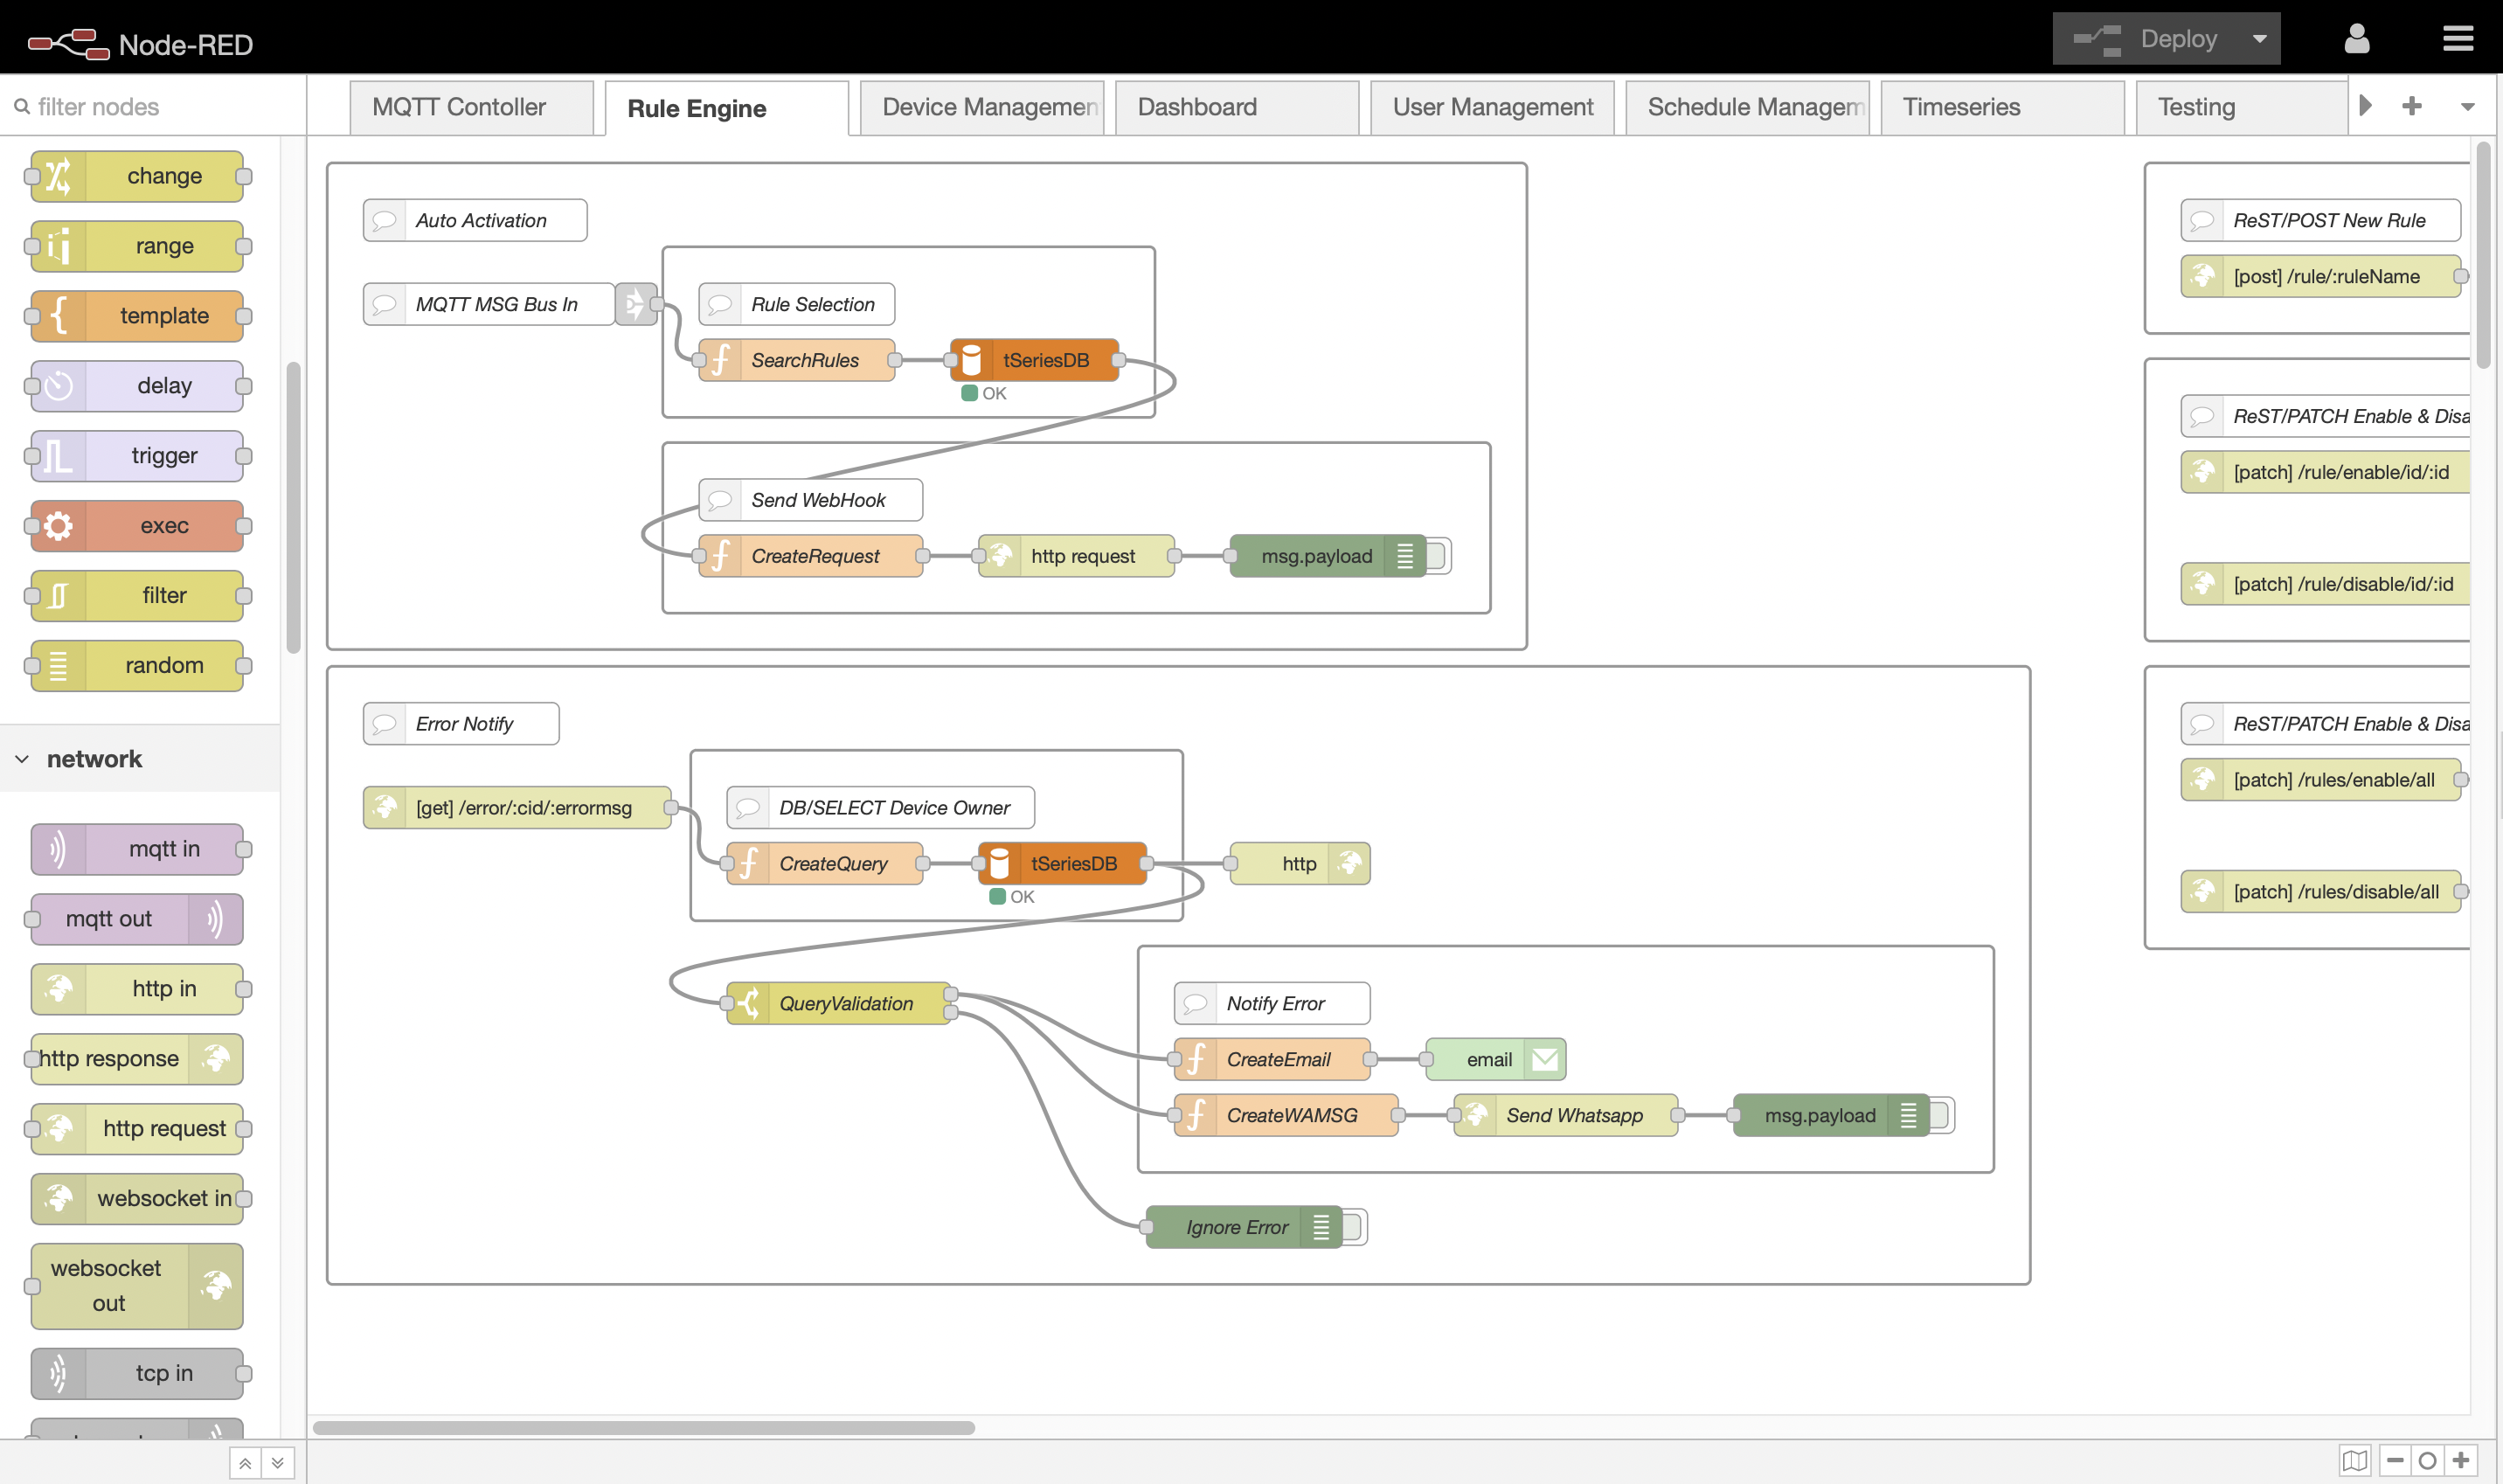
\includegraphics[width=0.5\textwidth]{./images/platformImpl.png}}
\caption{Node-RED screenshot for flow of platform}
\label{fig}
\end{figure}

\subsubsection{MQTT Controller}
MQTT Manager in the Node-RED is the gateway for MQTT messages to enter Node-RED. The main purpose of this block is to convert incoming MQTT messages to give convenience to other Node-RED-based blocks. To achieve it, this block receives all the messages by subscribing to all the MQTT message topics. And then it parses message topic and payload to provide useful information such as the MQTT username and client id. These pieces of information are used in other Node-RED-based nodes in further progress.

\subsubsection{Rule Engine}
The purpose of Rule Engine is to activate actions according to MQTT messages. It cooperates with the Rule Table of Database to activate the action. Designing logic of the Rule Engine is inspired by the book, “Build Your Own IoT Platform” \cite{b22}. For every published message, Rule Engine searches for all rules where the rule’s message pattern satisfies the message content. Actions that corresponded to the rules are defined as ReST API form, thus activating action will be progressed as sending an HTTP request. It also provides ReST APIs for adding, modifying, and deleting rules. Some ReST APIs for actions are defined in another block, whereas some APIs are defined in Rule Engine, such as sending notifications.

\subsubsection{Device Manager}
Handling devices that are attached to the platform by users is the main purpose of the Device Manager block. It provides ReST APIs that can add a new device to the platform (with HTTP POST method), modify the status of the device (with HTTP PATCH method), delete a device (with HTTP DELETE method). And it also provides functionality for publishing an action-type message to a specific device.

\subsubsection{Dashboard}
Dashboard Manager is to provide Graphical User Interface (GUI) to the user. By using this block, users can be provided the status of water and food remaining and consumption visually. It also provides buttons to serve food and input areas to set user settings.

\subsubsection{User Management}
The purpose of the User Manager block is to provide an interface for modifying user settings. Users can manage these 4 settings: Notification, Email address, WhatsApp information, and timezone where the user lives.  To support global users, Timezone settings are included. As all the times that platform uses and database stores use Coordinated Universal Time (UTC) timezone, converting the time of the user to the UTC is necessary. This setting is especially important when a user adds a new schedule by using Schedule Engine, and when providing local time to the user in the Dashboard.

\subsubsection{Schedule Engine}
Handling and executing schedules is the main functionality for this block. For schedule execution, it cooperates with the Schedule Table in the Database. Every minute, the Schedule Engine checks the Schedule Table and executes the actions that are scheduled to be activated at that time. Also, this block provides ReST APIs that can create, read, update and delete the schedule.

\subsubsection{Timeseries Manager}
Managing Time-series Data Table of Database is the main purpose for Time-series Manager block. This block provides 3 types of ReST APIs for managing time-series data: Inquiring record feature (with HTTP GET method), Changing record validity (with HTTP PATCH method), and Deleting record (with HTTP DELETE method).

% ::—— Dashboard Implementation ——::
\subsection{Dashboard}
Petification’s dashboard was implemented using ‘node-red-dashboard’, which provides a set of nodes to make a live data dashboard \cite{b23}.
The dashboard consists of three tabs: Feed Machine tab, Water Supplier tab, and User Settings tab.

% ::Feed Machine tab::
\subsubsection{Feed Machine tab}
In the Feed Machine tab, Device Information widget, Feed Machine Statistics widget, and Serve Food widget are provided. As all the functionalities this tab provides are device-specific, selecting a device is included in the Device Information widget and is displayed as a dropdown.
% ::Device connectivity::
Also, the status for the selected device is provided in the text and LED-shaped icon. The color of the LED-shaped icon changes to green when the device is connected, red for disconnected status, and yellow for error status.

% ::Remaining of the food::
In the Feed Machine Statistics widget, the Remaining amount of food and container and food consumption is provided. The remaining amount of food bowl and container is displayed as gauge and food consumption is displayed as a line graph.

% ::Serve food by button or schedule::
In the Serve Food widget, the user input interface is provided to publish feed serving action by button. The serve Food widget also provides the interface for automatic food feeding (scheduled feeding). Users can see all the feeding schedules in the table format, add a new schedule by user input interface, and delete the existing schedule by clicking the row of the table. Figure 14 shows the screenshot of implemented Feed Machine tab.

\begin{figure}[htbp]
\centerline{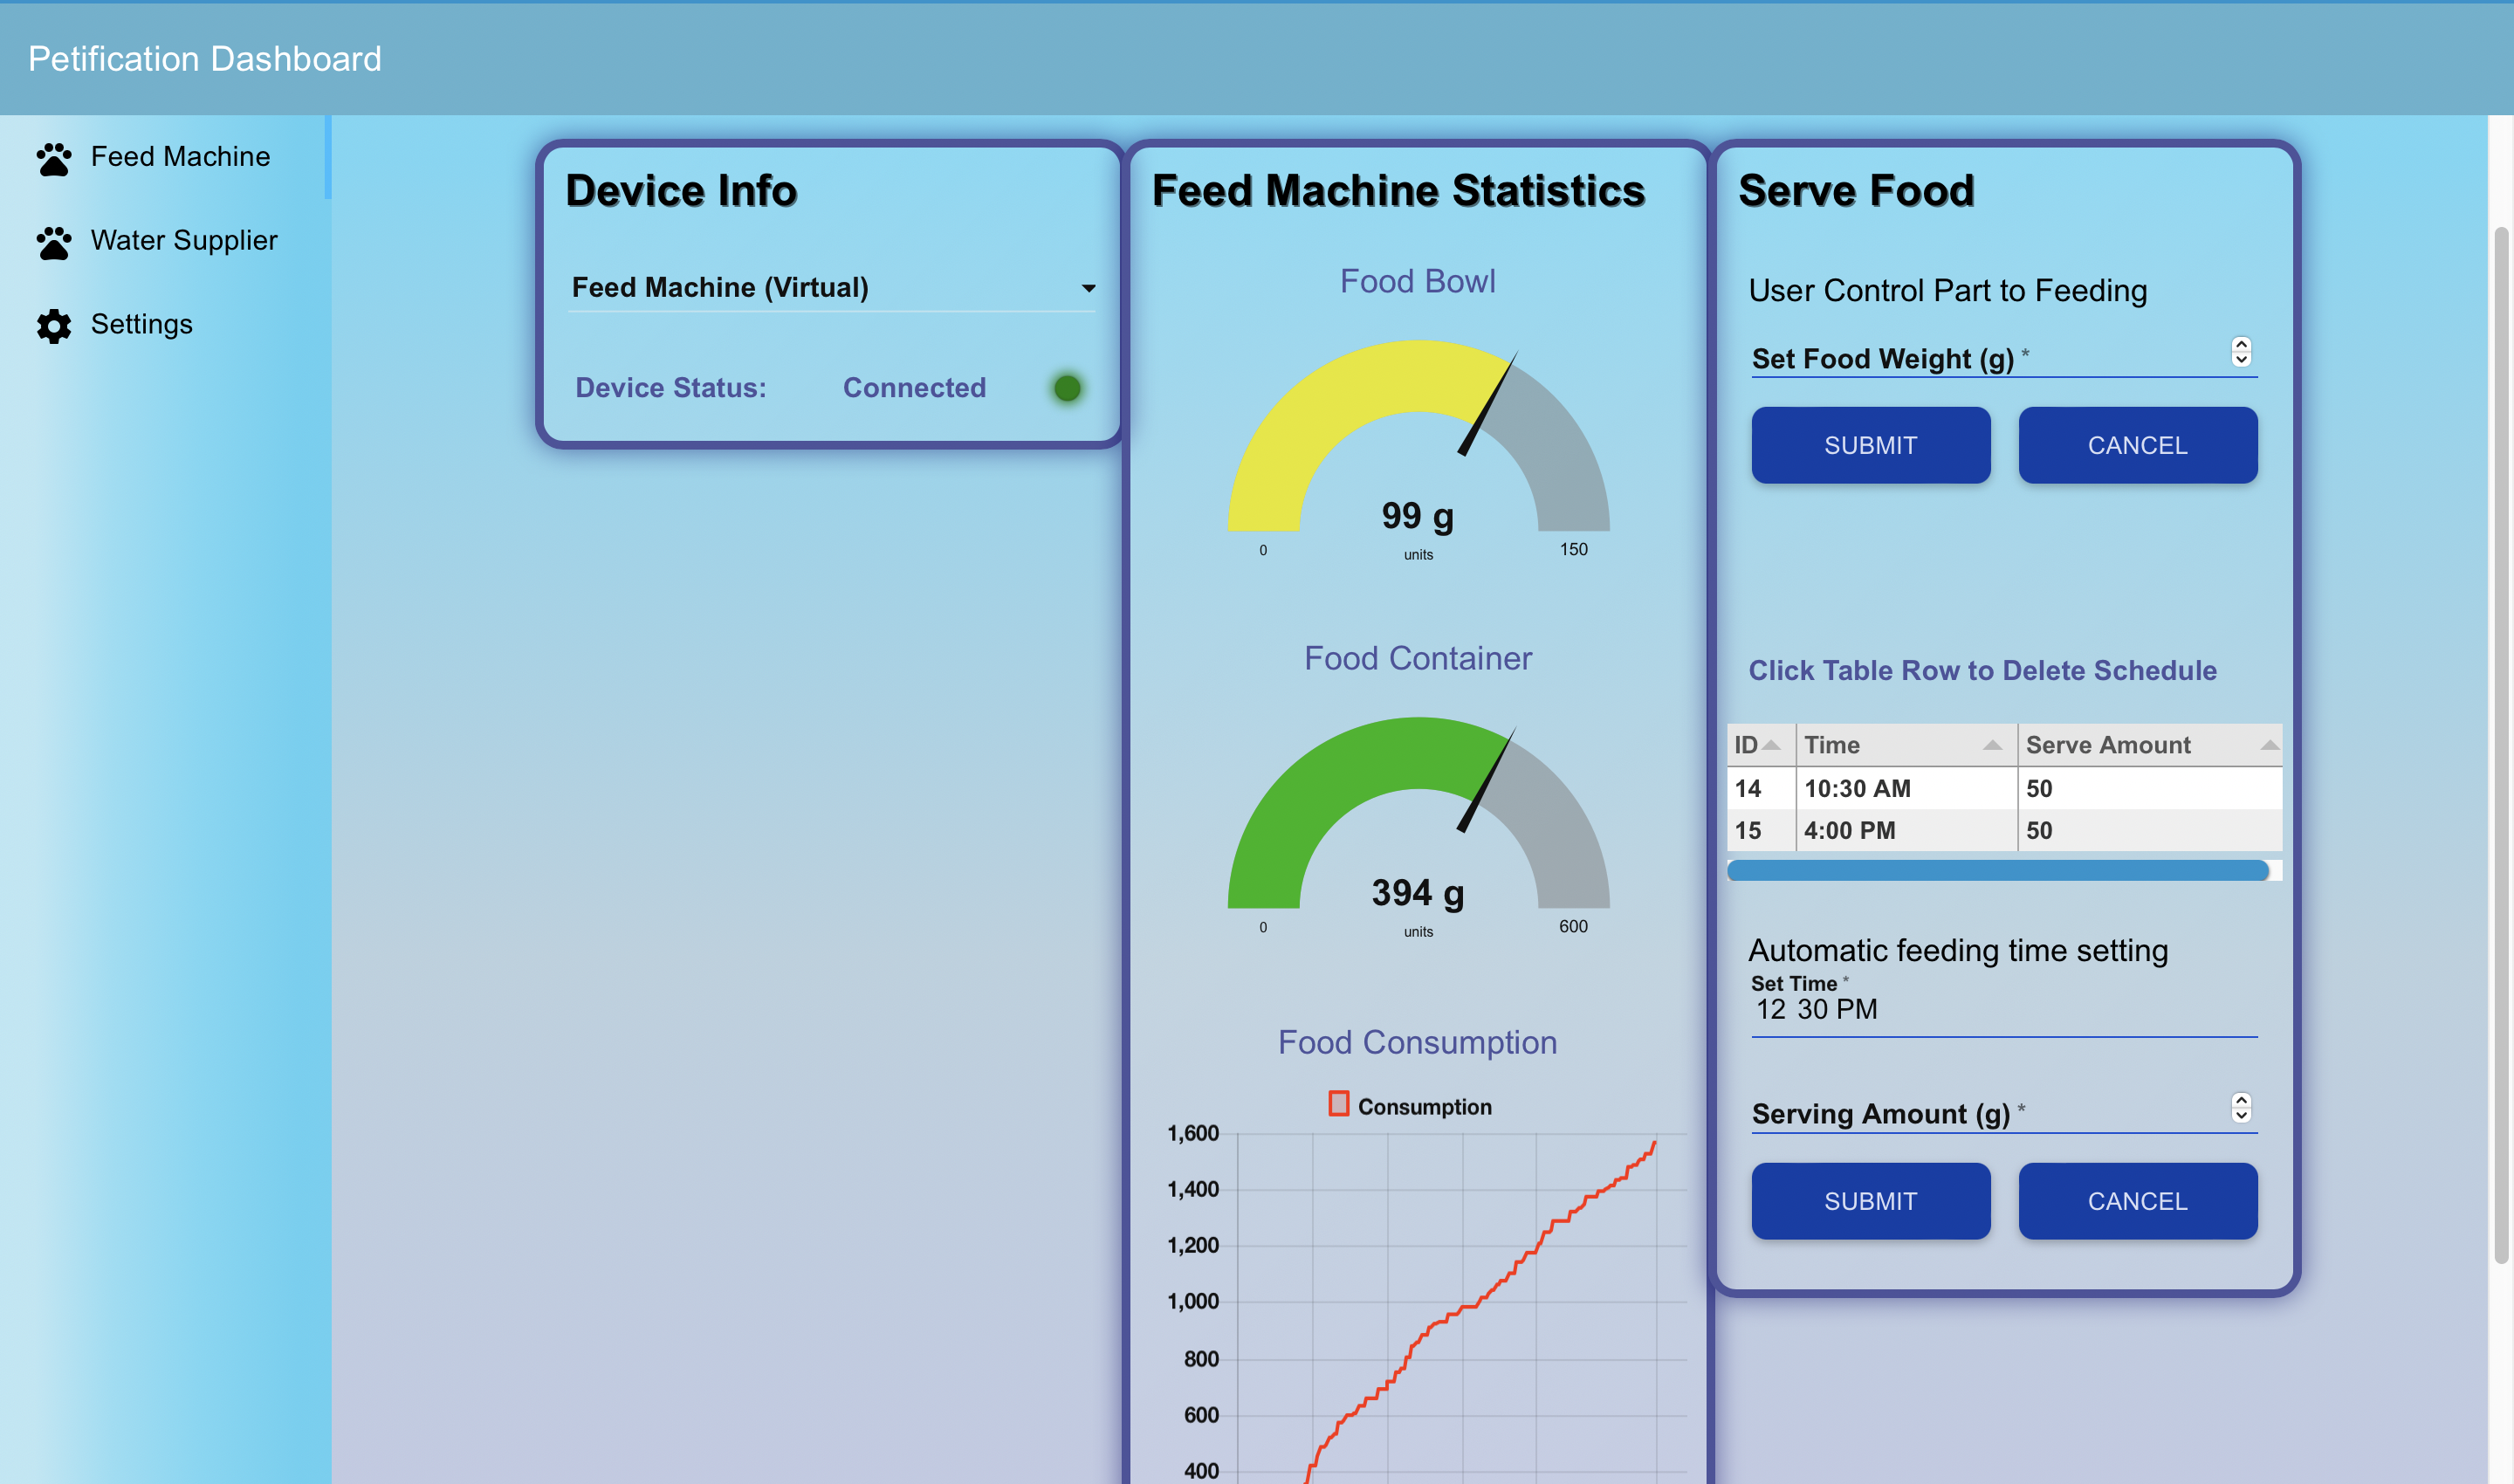
\includegraphics[width=0.5\textwidth]{./images/feed_machine_ui.png}}
\caption{Screenshot for Feed Machine tab}
\label{fig}
\end{figure}

% ::Water Supplier tab::
\subsubsection{Water Supplier tab}
Similar to the Feed Machine tab, the Water Supplier tab provides two widgets: Device Information widget and Water Supplier Statistics widget. The mechanism for each widget is identical to the Feed Machine tab. Figure 15 shows the screenshot of implemented Water Supplier tab.

\begin{figure}[htbp]
\centerline{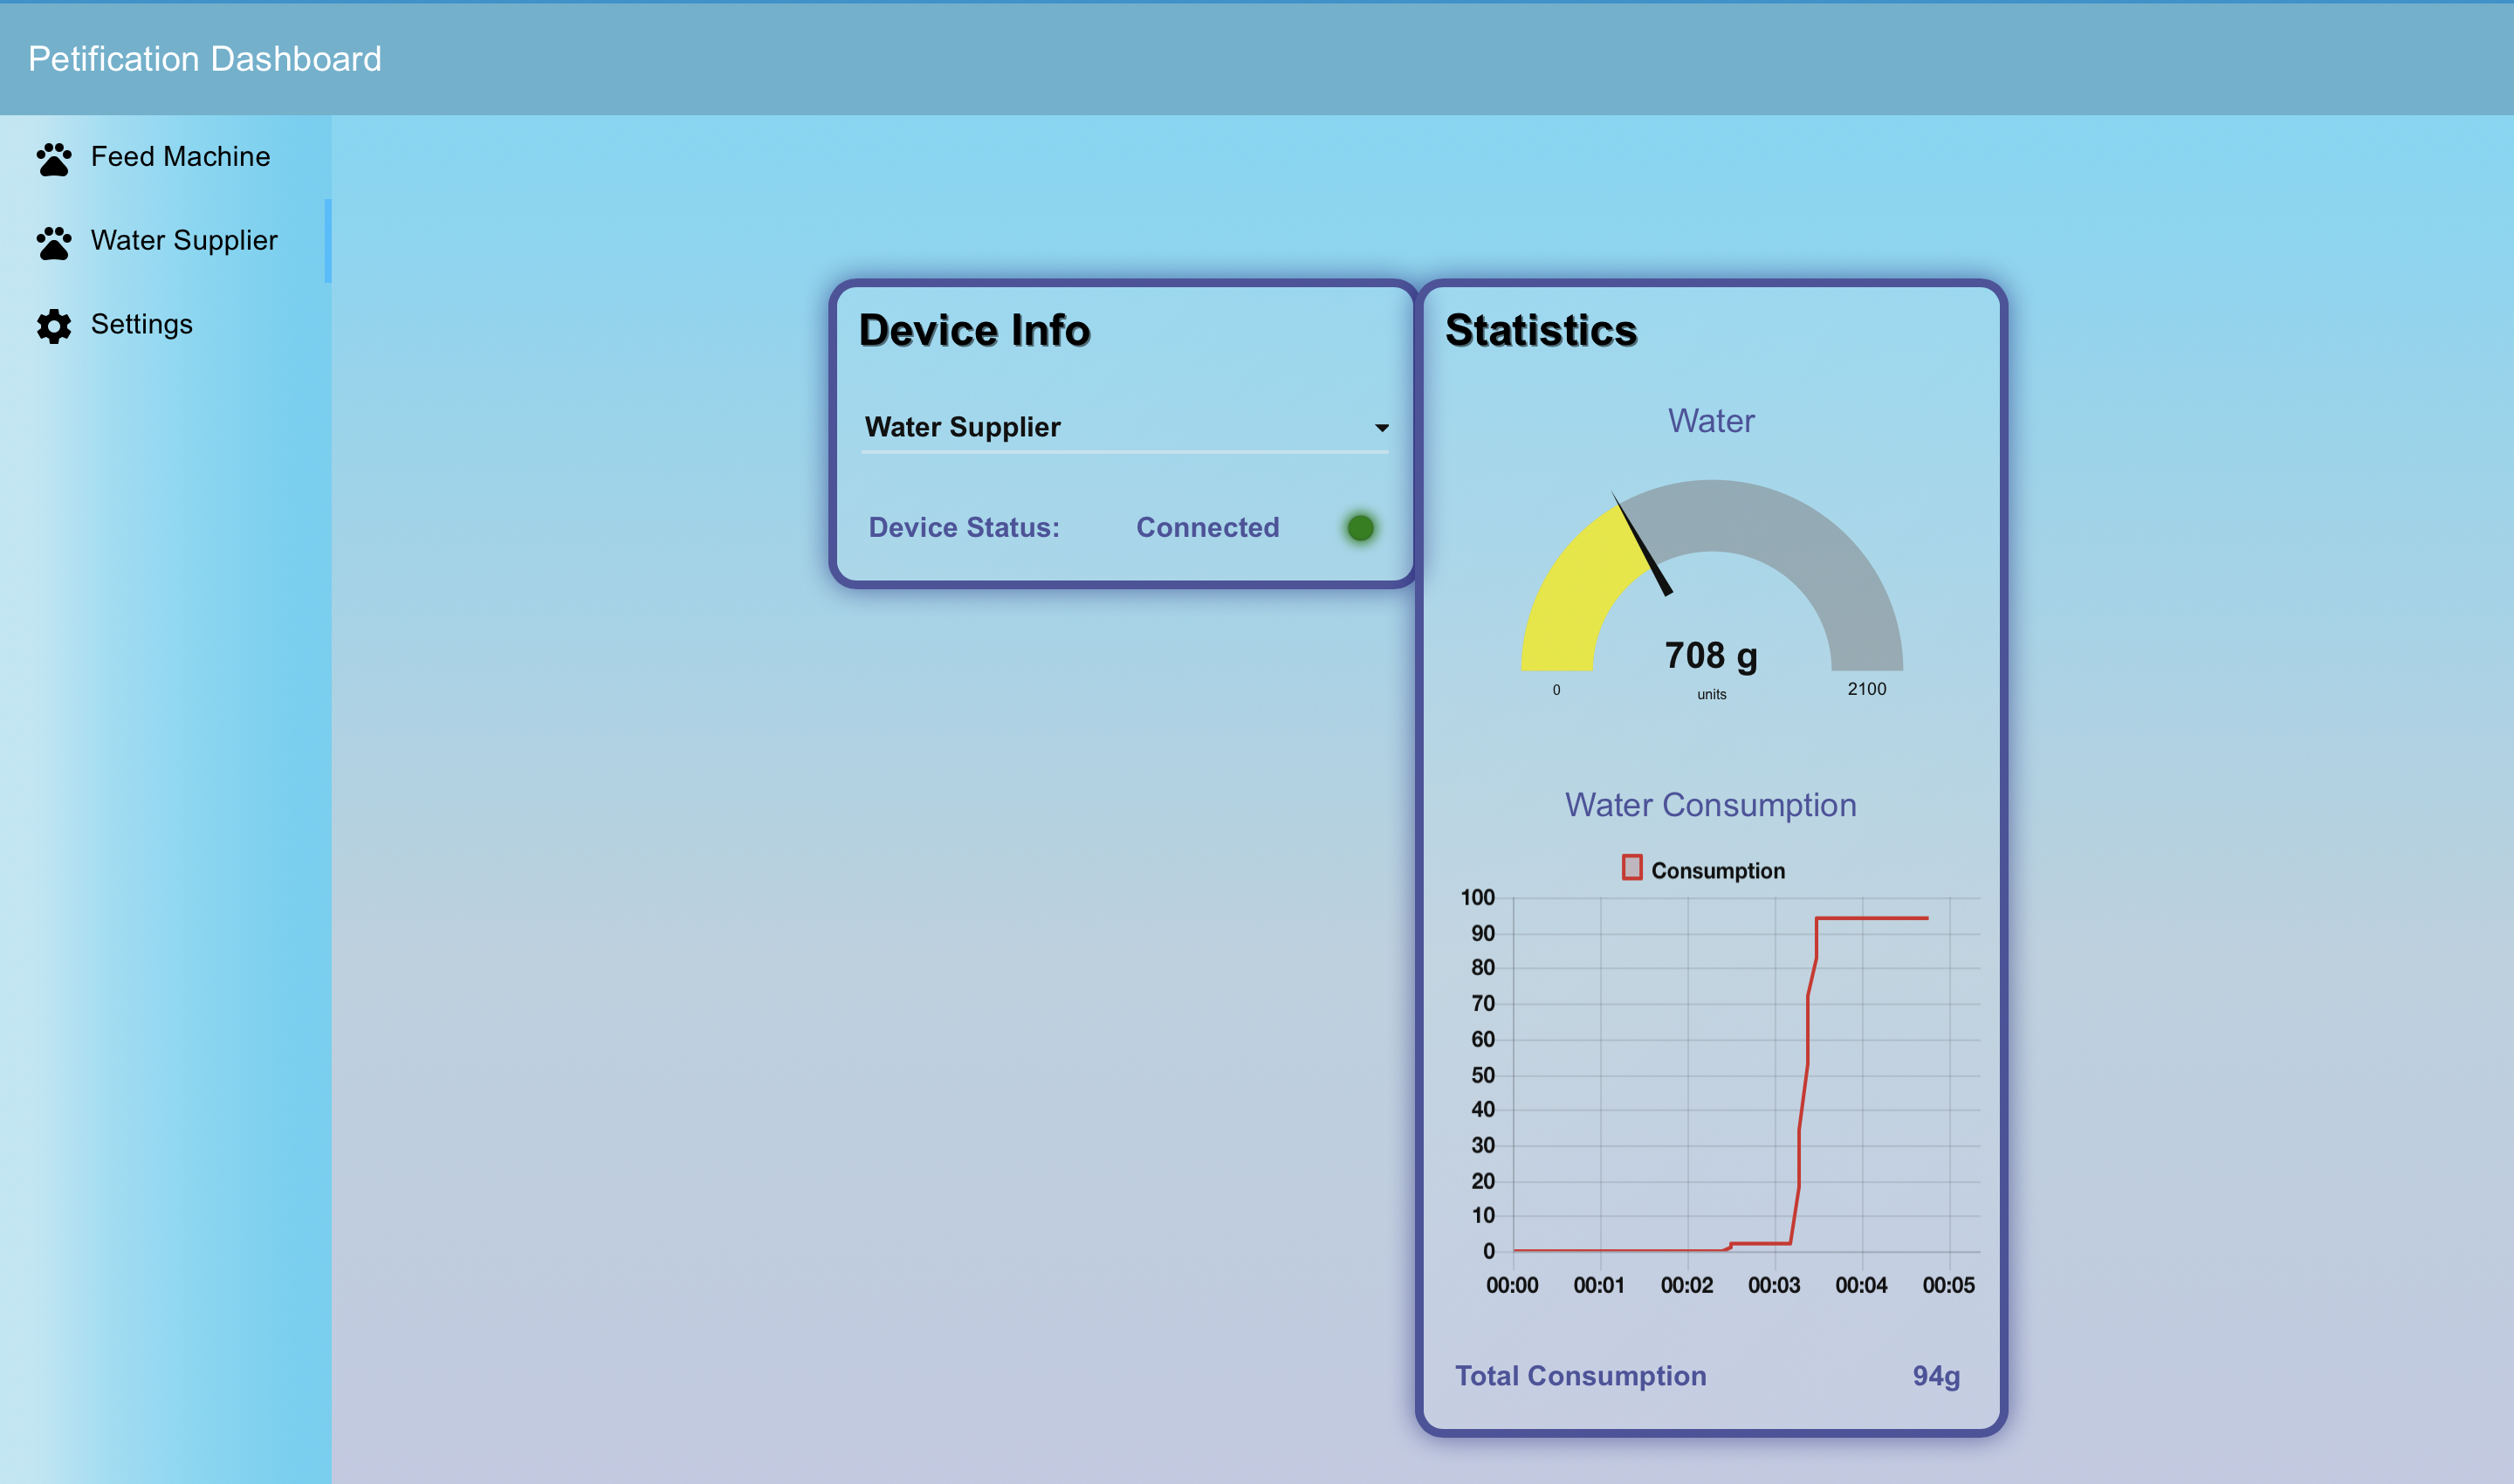
\includegraphics[width=0.5\textwidth]{./images/water_supplier_ui.png}}
\caption{Screenshot for Water Supplier tab}
\label{fig}
\end{figure}

% ::User Settings tab::
\subsubsection{User Settings tab}
The User Settings tab provides five widgets: User Information widget, Timezone settings widget, Notification settings widget, E-Mail address settings widget, and WhatsApp settings widget. 
% ::Sign in by token::
In the User Information widget, users can sign in to the system by entering the token, which is an identifier for the user. After signing in, the user can see the token and username of the current user.
% ::Set timezone::
To support global users, the Timezone settings widget is included in the tab. As all the times that platform uses and database stores use Coordinated Universal Time (UTC) timezone, converting the time of the user to the UTC is necessary.
% ::Notification option::
Notification settings widget, E-Mail address settings widget, and WhatsApp settings widget are to control error notification. Users can turn notifications on and off with the Notification settings widget and decide which accounts receive email and WhatsApp messages. Figure 16 shows the screenshot of the implemented User Settings tab.

\begin{figure}[htbp]
\centerline{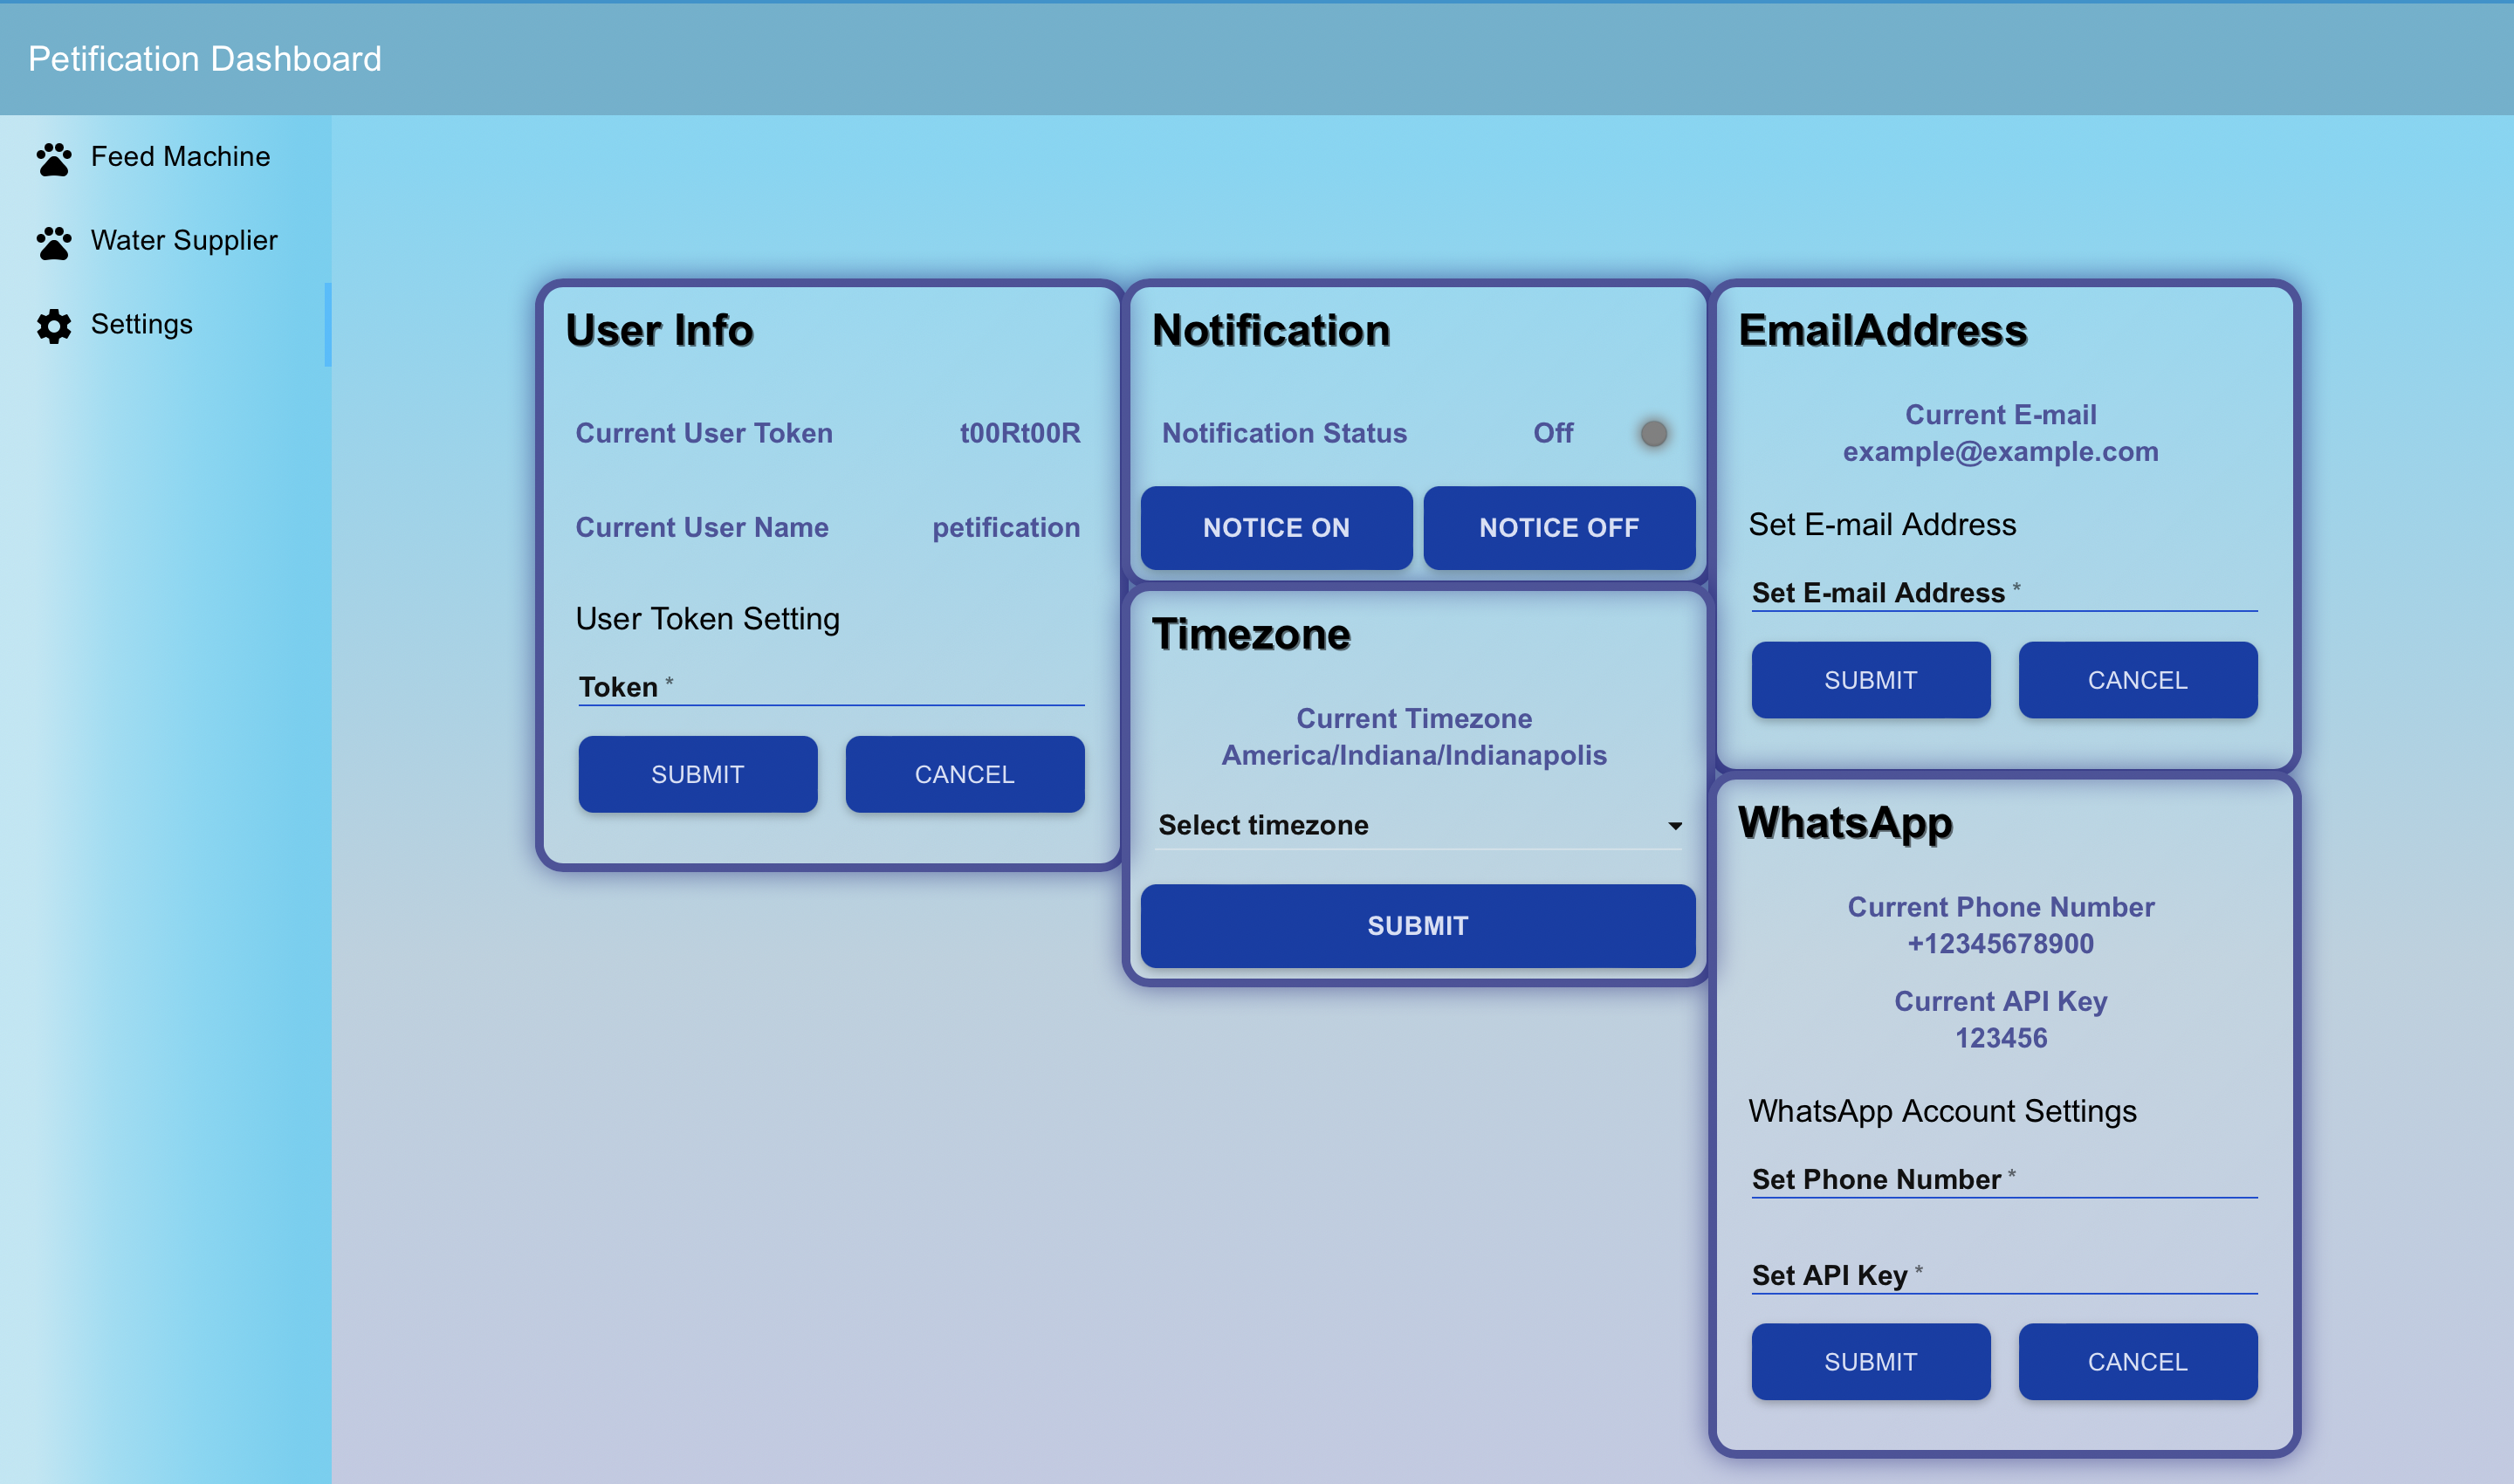
\includegraphics[width=0.5\textwidth]{./images/user_settings_ui.png}}
\caption{Screenshot for User Settings tab}
\label{fig}
\end{figure}

% ::—— EXPERIMENT & TESTING ——::
\section{Experiment and Testing}
Testing is conducted based on the results of the implementation of the Petification IoT Platform. Testing is conducted only on quantitatively verifiable results, and a total of two cases are covered: accuracy testing of the weight measurement and that of the automatic feeding.

% ::Weight measurement testing::
\subsection{Weight measurement testing}
In this test, a total of 8 tests were performed using a load cell sensor in which calibration was completed, and actual weight is compared with the measured weight in each test.

\begin{figure}[htbp]
\centerline{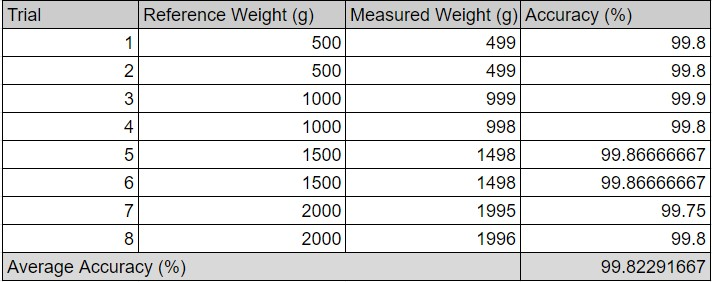
\includegraphics[width=0.5\textwidth]{./images/Calibration_sheet.jpg}}
\caption{Testing result of weight measurement}
\label{fig}
\end{figure}

It was confirmed that the average accuracy was 99.8\%, which resulted in high accuracy. Through this, it can be confirmed that the weight measurement error by the sensor hardly occurs as the result of subsequent testing.

% ::Automatic feeding testing::
\subsection{Automatic feeding testing}
In this test, a total of 10 tests were performed to figure out the automatic feeding feature works as expected. The desired serving amount is compared with the actual serving amount in each test.

\begin{figure}[htbp]
\centerline{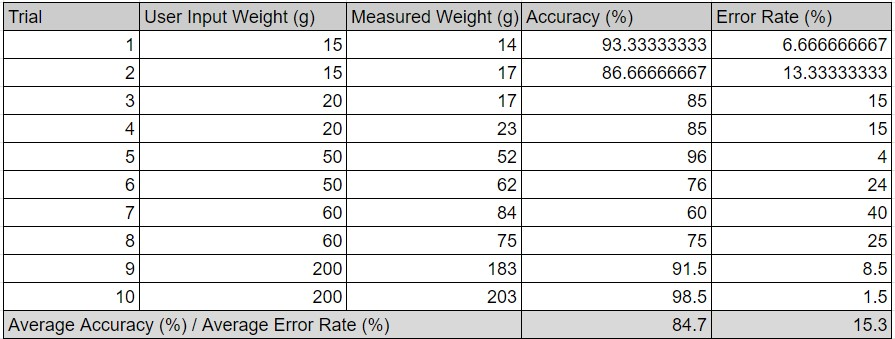
\includegraphics[width=0.5\textwidth]{./images/Feeding_sheet.jpg}}
\caption{Testing result of automatic feeding}
\label{fig}
\end{figure}

As a result of the measurement, it was confirmed that 40\% of the highest error was found, and 1.5\% of the lowest error was found. The reason for the error is that the food is often stuck in front of the food gate and the food serving speed is too fast for the load cell to detect. It is a limitation for the feed machine and can be solved if the design is modified correctly.

% ::—— CONCLUSION ——::
\section{Conclusion}
In the present research, a pet-care IoT solution named ‘Petification’ is proposed to take care of users’ pets when they are not at home. The water supplier is supported in the petification to supply water to the pet and report the current amount of the remaining water. The feed machine is also supported to serve a certain amount of food to the pet and report the current amount of the remaining food. The IoT platform for Petification is implemented using Node-RED to take advantage of open-source and flow-based visual programming. Also, the message flow for the Petification is controlled with Eclipse Mosquitto, which is an open-source implementation of the MQTT Protocol. Users for this solution can check the water and food consumption of the pet and serve the food to the pet on the web-based dashboard. The dashboard of the petification also provides device connectivity and the amount of remaining food and water to the user. When the water or food for each device is empty, the user can get notifications for it.

% ::Limitations and future plans::
While all other functionalities are working correctly, the accuracy of serving the exact amount of food to the pet is relatively low. The low accuracy is caused by the design of the food gate and the sensitivity of the load cell. Thus, the future plan can be enhancing the design of the food gate and the sensitivity and stability of the load cell to serve the exact amount of food. Also, attaching another type of device such as a device for taking pictures of the pet can be a possible improvement for Petification.

% ::—— ACKNOWLEDGEMENT ——::
\section{Acknowledgement}
“This research was supported by the MSIT(Ministry of Science and ICT), Korea, under the National Program for Excellence in SW) supervised by the IITP(Institute of Information \& communications Technology Planing \& Evaluation) in 2021”(2021-0-01435)
The authors of this study are grateful to Professor Minsun Lee of Chungnam National University, Professor Eric T. Matson, Professor Anthony H. Smith, and Teaching Assistant Minji Lee of Purdue University for helping us participate in the project.

\begin{thebibliography}{00}
\bibitem{b1} 
M.  Hanson.  “Pet  Industry  Statistics”  spots.com.  https://spots.com/pet-industry-statistics/ (accessed Jan. 25, 2022). 
\bibitem{b2}
Accessed: Feb. 1, 2022. [Online]. Available: https://www.instructables.com/IOT-Pet-Feeder-Using-the-Blynk-Mobile-App-an-ESP82/
\bibitem{b3}
Accessed: Feb. 1, 2022. [Online]. Available: https://www.instructables.com/IoT-Pet-Feeder/
\bibitem{b4}
T. Sangvanloy and K. Sookhanaphibarn, "Automatic Pet Food Dispenser by using Internet of Things (IoT)," 2020 IEEE 2nd Global Conference on Life Sciences and Technologies (LifeTech), Kyoto, Japan, Mar. 10-12, 2020.
\bibitem{b5}
Y. Chen and M. Elshakankiri, "Implementation of an IoT based Pet Care System," 2020 Fifth International Conference on Fog and Mobile Edge Computing (FMEC), Paris, France, Apr. 20-23, 2020.
\bibitem{b6}
Accessed: Feb. 4, 2022. [Online]. Available: https://iotdesignpro.com/projects/google-assistant-controlled-iot-pet-feeder-using-esp8266
\bibitem{b7}
Accessed: Feb. 5, 2022. [Online]. Available: https://create.arduino.cc/projecthub/circuito-io-team/iot-pet-feeder-10a4f3
\bibitem{b8}
Node-RED [Online]. Available: https://nodered.org/about/
\bibitem{b9}
MQTT [Online]. Available: https://mqtt.org
\bibitem{b10} %10
P. N. Vrishanka, P. Prabhakar, D. Shet and K. Rupali, "Automated Pet Feeder using IoT," 2021 IEEE International Conference on Mobile Networks and Wireless Communications (ICMNWC), Tumkur, Karnataka, India, Dec. 3-4, 2021.
\bibitem{b11} %11
R. Nogueira, H. Araújo and D. Prata. (Apr. 2019). Robot Chow: Automatic Animal Feeding with Intelligent Interface to Monitor Pets. International Journal of Advanced Engineering Research and Science. [Online]. Available: https://ijaers.com/detail/robot-chow-automatic-animal-feeding-with-intelligent-interface-to-monitor-pets/
\bibitem{b12} %12
Vania, K. Karyono and I. H. T. Nugroho, "Smart dog feeder design using wireless communication, MQTT and Android client," 2016 International Conference on Computer, Control, Informatics and its Applications (IC3INA), Tangerang, Indonesia, Oct. 3-5, 2016.
\bibitem{b13} %13
Thepihut. https://thepihut.com/blogs/raspberry-pi-roundup/whats-the-difference-between-dc-servo-amp-stepper-motors (accessed Feb. 04, 2022).
\bibitem{b14} %14
Accessed: Feb. 15, 2022. [Online]. Available: https://instrumentationtools.com/load-cell-working-principle/
\bibitem{b15} %15
Accessed: Feb. 19, 2022. [Online]. Available: https://www.seeedstudio.com/blog/2019/11/26/10-things-you-can-do-with-your-hx711-and-load-cell/
\bibitem{b16} %16
Accessed: Feb. 6, 2022. [Online]. Available: https://www.fujielectric.com/products/column/servo/servo\_01.html
\bibitem{b17} %17
N. B. Kamarozaman and A. H. Awang, "IOT COVID-19 Portable Health Monitoring System using Raspberry Pi, Node-Red and ThingSpeak," 2021 IEEE Symposium on Wireless Technology \& Applications (ISWTA), Shah Alam, Malaysia, Aug. 17-17, 2021.
\bibitem{b18} %18
N. Naik, "Choice of effective messaging protocols for IoT systems: MQTT, CoAP, AMQP and HTTP," 2017 IEEE International Systems Engineering Symposium (ISSE), Vienna, Austria, Oct. 11-13, 2017.
\bibitem{b19} %19
OASIS Open [Online]. Available: https://www.oasis-open.org/committees/tc\_home.php?wg\_abbrev=mqtt
\bibitem{b20} %20
Eclipse Mosquitto [Online]. Available: https://mosquitto.org/
\bibitem{b21} %21
Datamation. [Online]. Available: https://www.datamation.com/storage/8-major-advantages-of-using-mysql/
\bibitem{b22} %22
A. Tamboli, “Build Your Own IoT Platform,” in \textit{Apress}, 1st ed, 2019
\bibitem{b23} %23
Node-RED [Online]. Available https://flows.nodered.org/node/node-red-dashboard

\end{thebibliography}
\vspace{12pt}
\end{document}
